\documentclass[10pt,a4paper]{scrartcl}

\usepackage[ngerman]{babel}

\input{../../Headerfiles/Packages}
\input{../../Headerfiles/Titles}
\input{../../Headerfiles/Commands}

%-------------------------------------------------------------------
%\linespread{1}
\renewcommand{\baselinestretch}{1.3}
%-------------------------------------------------------------------

\author{GianAndrea Müller, nach der Vorlesung von Prof. Dr. W. Wegscheider}
\title{Zusammenfassung Physik I\&II}
\begin{document}
	
 	\maketitle
 	\begin{multicols*}{4}
 	\setcounter{tocdepth}{2}
 	\scriptsize
 	\tableofcontents
 	\normalsize
 	\end{multicols*}
 	\clearpage
 	
 	\parindent 0pt %no indent at the first line of a new paragraph
	\setlength{\columnseprule}{1pt}
 
\begin{multicols*}{2}

 	\section{Konstanten}
 	
 	\begin{tabular}{p{0.36\linewidth}p{0.08\linewidth}p{0.45\linewidth}}
	\hline
 	Konstante				&	Symbol		&		Wert\\
	Dielektrizitätskonstante&	$\epsilon_0$ &		\SI{8.854188e-12}{\coulomb\squared\second\squared\per\kilogram\per\meter\cubed}\\
							&	$4\pi\epsilon_0$&	\SI{1.112650e-10}{\coulomb\squared\second\squared\per\kilogram\per\meter\cubed}\\	
 	Elementarladung			&	$e$			&		\SI{1.60219e-19}{\coulomb}\\
 	Magnetische Feldkonstante&	$\mu_0$		&		\SI{4\pi e-7}{\newton\per\ampere\squared}\\
 	Lichtgeschwindigkeit im Vakuum&	$c$			&		\SI{2.997925e8}{\meter\per\second}\\
	Avogadro'sche Zahl 		& 	$N_0$		&		\SI{6.02205e23}{\per\mole} \\
	Planck'sche Konstante		&	$h$			&		\SI{6.62618e-34}{\joule\second}\\
							&	$\hbar$		&		\SI{1.05450e-34}{\joule\second}\\
	Atomare Masseneinheit		&	$amu$		&		\SI{1.66056e-27}{\kilogram}\\
	Elektronenmasse 		& 	$m_e$		&		\SI{9.10953e-31}{\kilogram}\\
	Protonenmasse		&	$m_p$		&		\SI{1.67265e-27}{\kilogram}\\
	Boltzmannkonstante		&	$k_B$		&		\SI{1.38066e-23}{\kilogram}\\
	Molare Gaskonstante 		&	$R$			&		\SI{8.31441}{\joule\per\kelvin\per\mole}\\
	Rydbergkonstante		&				&\\
		(infinite nuclear mass)&	$R_\infty$&		\SI{2.179914e-23}{\joule}\\
	Erster Bohrradius		&	$a_0$		&		\SI{5.29177e-11}{\meter}\\
	Bohr magneton			&	$\mu_B$		&		\SI{9.27409e-24}{\joule\per\tesla}\\
	Stefan-Boltzmann Konstante&	$\sigma$	&		\SI{5.67032e-8}{\joule\per\meter\squared\per\kelvin\tothe{4}\per\second}
 	\end{tabular}
 
 	\section{Nice to know}
 	
 	$\expval{v}=\sqrt{\frac{8k_BT}{\pi m}}$	
 	
	\end{multicols*} 	
 	
	\begin{multicols*}{3}
	\small 
	
	\setlength{\columnseprule}{1pt}
 	
 	\section{Identitäten}
 	
 	\subsection*{le Logarithmus}
	$\ln(ab)=\ln(a)+\ln(b)$
	\subsection*{Derivatives}
	$(ln(x))'=\frac{1}{x}$
	\subsection*{Integrals}	
	$\int{ln(x)}dx =x\cdot ln(x) -x + C$
	
	$\int{e^xdx}=e^x$ \hfill $\int{a^xdx}=\frac{a^x}{\ln(a)}+C$
	
	$\int{\frac{1}{\cos^2(x)}dx}=\tan(x)+C$
	
	$\int{\frac{1}{\sin^2(x)}dx}=-\cot(x)+C$
	
	\finn
	
	$\int{\sin^2(x)dx}=\frac{1}{2}(\sin(x)\cos(x)-x)+C$
	
	$\int{\cos^2(x)dx}=\frac{1}{2}(\sin(x)\cos(x)+x)+C$
	
	\finn
		
	$\int{\frac{1}{1+x^2}dx}=
	\begin{cases}
	\arctan(x)+C_1\\
	-arccot(x)+C_2
	\end{cases}$
	
	$\int{\frac{1}{1-x^2}}=
	\begin{cases}
	$artanh$(x)+C_1=\frac{1}{2}\ln(\frac{1+x}{1-x}+C_1)&	|x|<1\\
	$arcoth$(x)+C_2=\frac{1}{2}\ln(\frac{x+1}{x-1}+C_2)&	|x|>1
	\end{cases}$
	
	\finn
	
	$\int{\frac{1}{\sqrt{1-x^2}}dx}=
	\begin{cases}
	\arcsin(x)+C_1\\
	-\arccos(x)+C_2
	\end{cases}	
	$
	
	$\int{\frac{1}{\sqrt{x^2-1}}dx}=$arcosh$(x)+C=\ln|x+\sqrt{x^2-1}|+C$ \hfill $|x|>1$
	
	\finn
	
	$\int{\frac{1}{\sinh^2(x)}dx}=-\coth(x)+C$	
	
	$\int{\frac{1}{\cosh^2(x)}dx}=\tanh(x)+C$
	
	\finn
	
	$\int{\frac{1}{\sqrt{x^2+1}}dx}=$arsinh$(x)+C=\ln|x+\sqrt{x^2+1}|+C$
		
	$\int{\frac{1}{x^2+a^2}dx}=\frac{1}{a}\arctan(\frac{x}{a})+C$
	
	\finn
	
	$\int{\frac{1}{\left(z^2+^2\right)^{3/2}}dz}=\frac{z}{a^2\sqrt{z^2+a^2}}+C$
	
	\subsection*{Euleridentität}
	$\Im(e^{ix})=\sin(x)=\frac{e^{ix}-e^{-ix}}{2i}$ \hfill $e^{i\omega x}=\cos(\omega x)+i\sin(\omega x)$
	
	$\Re(e^{ix})=\cos(x)=\frac{e^{ix}+e^{-ix}}{2}$
	
	\columnbreak	
	
	\subsection*{Trigonometrie}
	
	$\sin^2(x)+\cos^2(x)=1$	

	\finn
	
	$\sin(\alpha \pm \beta)=\sin(\alpha)\cos(\beta)\pm \cos(\alpha)\sin(\beta)$
	
	$\cos(\alpha \pm \beta)=\cos(\alpha)\cos(\beta)\mp \sin(\alpha)\sin(\beta)$
	
	\finn	
	
	$\sin(\alpha)+\sin(\beta) = 2\sin(\frac{\alpha+\beta}{2})\cos(\frac{\alpha-\beta}{2})$
	
	$\sin(\alpha)-\sin(\beta)=2\cos(\frac{\alpha+\beta}{2})\sin(\frac{\alpha-\beta}{2})$
	
	$\cos(\alpha)+\cos(\beta)=2\cos(\frac{\alpha+\beta}{2})\cos(\frac{\alpha-\beta}{2})$
	
	$\cos(\alpha)-\cos(\beta)=2\sin(\frac{\alpha+\beta}{2})\sin(\frac{\alpha-\beta}{2})$
	
	\finn
	
	$\sin(2x)=2\sin(x)\cos(x)$
	
	$\sin(3x)=3\sin(x)-4\sin^3(x)$
	
	$\sin(4x)=\sin(x)(8\cos^3(x)+4\cos(x))$
	
	$\sin(5x)=5\sin(x)-20\sin^3(x)+16\sin^5(x)$
	
	\finn
	
	$\cos(2x)=\cos^2(x)-\sin^2(x)=1-2\sin^2(x)$
	
	$\cos(3x)=4\cos^3(x)-3\cos(x)$
	
	$\cos(4x)=8\cos^4(x)-8\cos^2(x)+1$
	
	$\cos(5x)=16\cos^5(x)-20\cos^3(x)+5\cos(x)$
	
	\finn
	
	$\tan(2x)=\frac{2\tan(x)}{1-\tan^2(x)}$
	
	$\tan(3x)=\frac{3\tan(x)-\tan^3(x)}{1-3\tan^2(x)}$
	
	\finn
	
	$\sin^2(x)=\frac{1}{2}(1-\cos(2x))$
	
	$\sin^3(x)=\frac{1}{4}(3\sin(x)-\sin(3x))$
	
	$\sin^4(x)=\frac{1}{8}(\cos(4x)-4\cos(2x)+3)$

	$\sin^n(x)=\frac{1}{2^n}\sum_{k=0}^n{{n\choose k} \cos((n-2k)(x-\frac{\pi}{2}))}$
	
	\finn
	
	$\cos^2(x)=\frac{1}{2}(1+\cos(2x))$
	
	$\cos^3(x)=\frac{1}{4}(3\cos(x)+\cos(3x))$
	
	$\cos^4(x)=\frac{1}{8}(3+4\cos(2x)+cos(4x))$
	
	$\cos^n=\frac{1}{2^n}\sum_{k=0}^n{{n\choose k}  \cos((n-2k)x)}$
	
	\finn
	
	$\sin(ax)\sin(bx)=\frac{1}{2} (\cos(x(a-b))-\cos(x(a+b)))$
	
	$\cos(ax)\cos(bx)=\frac{1}{2} (\cos(x(a-b))+\cos(x(a+b)))$
	
	$\sin(ax)\cos(bx)=\frac{1}{2} (\sin(x(a-b))+\sin(x(a+b))$
	
	\finn
	
	$\sinh(x)=\frac{e^x-e^{-x}}{2}$ \hfill $\cosh(x)=\frac{e^x+e^{-x}}{2}$
	
	$\cosh^2(x)-\sinh^2(x)=1$ \hfill $\cosh(x)+\sinh(x)=e^x$
	
	$\sinh(2x)=2\sinh(x)\cosh(x)$
	
	$\sinh(3x)=4\sinh^3(x)+3\sinh(x)$
	
	$\cosh(2x)=\cosh^2(x)+\sinh^2(x)=2\cosh^2(x)-1$
	
	$\cosh(3x)=4\cosh^3(x)-3\cosh(x)$
	\normalsize		
	
	\subsection{Differentialoperatoren}
	
	\begin{center}$f(\vec{r}):\mathbb{R}^3\longrightarrow\mathbb{R}^1\quad\vec{A}(\vec{r}),\vec{B}(\vec{r}):\mathbb{R}^3\longrightarrow\mathbb{R}^3$\end{center}
	
	\finn
	
	$\rota\vec{\nabla}f=0$\hfill$\rota(\dive f)=0 $\hfill$\dive(\rota\vec{A})=0$
	
	$\dive\dive f=\vec{\nabla}^2\cdot f=\vec{\Delta}\cdot f$
	
	$\dive(f\cdot\vec{A})=f\cdot(\dive\vec{A})+\vec{A}(\dive f)$
	
	$\dive(\Vprod{A}{B})=\vec{B}(\rota\vec{A})-\vec{A}(\rota\vec{A})$
	
	\finn
	
	Potentialfeld:$\quad\rota\vec{A}=0\Rightarrow\vec{A}=\dive f$ 
	
	quellenfrei:$\quad\dive\vec{A}=0$ \hfill rotationsfrei:$\quad\rota\vec{A}$
	
	\vfill
	
	\clearpage
	
	\section{Elektrizität}
	
	\subsection{Coulombkraft}
	
	$\vec{F} = \frac{1}{4\pi\epsilon_0}	Q_0Q_1	\frac{\vec{r_0}-\vec{r_1}}{|\vec{r_0}-\vec{r_1}|^3}	 =	\frac{1}{4\pi\epsilon_0}	Q_0Q_1	\frac{\vec{e_r}}{r^2}$ \hfill $[F]=N$
	
	$\vec{F}	=	\frac{Q_0}{4\pi\epsilon_0} \int_V{\rho(\vec{r'})	\frac{\vec{r_0}-\vec{r'}}{|\vec{r_0}-\vec{r'}|^3}dV'}$
	
	\subsection{Elektrisches Feld}
	
	\emph{Das Elektrische Feld ist gleich der Kraft, die auf eine positive Einheitsladung wirkt.} 
	
	\finn
	
	$\Eofr = \frac{\Fofr}{Q_0}$ \hfill $[\vec{E}]=\si{\volt\per\meter}=\si{\newton\per\coulomb}$
	
	$\Eofr=\frac{1}{4\pi\epsilon_0}\int_V{\rho(\vec{r'})\frac{\vec{r_0}-\vec{r'}}{|\vec{r_0}-\vec{r'}|^3}dV'}$
	
	\vspace{1ex}
	Beispiele von elektrischen Feldern:
	
	\begin{tabular*}{\linewidth}{l|l}
	\hline\\
	nichtleitende Kugel aussen&$\Eofr=\frac{Q_{Kugel}}{4\pi\epsilon_0r^2}^*$\\
	\hline\\
	nichtleitende Kugel innen&$\Eofr=\frac{Q_{Kugel}\cdot r}{4\pi\epsilon_0R^3}$\\
	\hline\\
	ebene Platte&$\Eofr=\frac{\sigma}{2\epsilon_0}$\\
	\hline\\
	langer Draht&$\Eofr=\frac{\lambda}{2\pi\epsilon_0r}$\\
	\hline
	\end{tabular*}

	\note{$^*$wie Punktladung}
	
	\subsection{Feldlinien} 
	
	Von \textcircled{+} nach \textcircled{-}, Anzahl Feldlinien $\propto$ Ladung. Dichte der Feldlinien $\propto |\vec{E}|$.
	
	\subsection{Elektrisches Dipolmoment} 
	
	$\vec{p}= Q2\vec{d}$\hfill $[\vec{p}] = \mathrm{1\,Debye} = \SI{3.335e-30}{\coulomb\meter}$
	
	\note{wobei 2$\vec{d}$ den Abstand der Ladungen bezeichnet.}
	
	$\vec{M} = \vec{p}\times\vec{E_0}$ \hfill $E_{el}=-\vec{p}\cdot\vec{E_0}$
	
	\subsection{Dipolfeld}
	
	$\Eofr = \frac{1}{4\pi\epsilon_0}\left[(+Q)\frac{\vec{r}-\vec{d}}{|\vec{r}-\vec{d}|^3}+(-Q)\frac{\vec{r}+\vec{d}}{|\vec{r}+\vec{d}|^3}\right]$
	
	$\Eofr \approx -\nabla(\frac{1}{4\pi\epsilon_0}\frac{\vec{p}\cdot\vec{r}}{|\vec{r}|^3})=\frac{1}{4\pi\epsilon_0}(\frac{3( \vec{p}\cdot\vec{r} )\cdot\vec{r}}{|\vec{r}|}-\frac{\vec{p}}{|\vec{r}|^3})$
	
	\note{Annäherung als Gradient eines Dipols gilt falls $|\vec{d}|\ll|\vec{r}|$.}
	
	\subsection{Elektrischer Fluss}
	
	$\Phi_E= \int_A{\Eofr\cdot d \vec{A'}}$ \hfill $[\Phi_E]=\mathrm{1\,\frac{Nm^2}{C}}$
	
	$\Phi_E \propto$ Anzahl Feldlinien, die durch A gehen.
	
	Im homogenen Feld $\Phi_E = \vec{E}\cdot\vec{A}$
	
	\subsection{Gesetz von Gauss}
	
	$\oint\limits_{A}{\Eofr\cdot d \vec{A'}}=\frac{Q}{\epsilon_0}=\frac{1}{\epsilon_0}\sum\limits_{i}Q_i=\frac{1}{\epsilon_0}\int\limits_V\rho(\vec{r}')dV'$
	
	In V eingeschlossene Gesamtladung $\propto$ Anzahl herauslaufende - Anzahl hineinlaufende Feldlinien.	
	
	\subsection{Anwendung: Satz von Gauss}
	
	$\oint_A{\Eofr\cdot d \vec{A}}\longeq
	\int_V{\vec{\nabla}\cdot\Eofr dV}\longeq
	\frac{1}{\epsilon_0}\int_v{\rho(\vec{r})dV}$
	
	\importname{Differentialform des Gesetz von Gauss}{$\vec{\nabla}\cdot\vec{E}=\frac{\rho}{\epsilon_0}$}
	
	\subsection{Elektrostatische Energie}	
	
	$E_{el} =-\int_{\vec{r_1}}^{\vec{r_2}}
	{\vec{F}(\vec{r})\cdot d \vec{r}}=
	-\int_{\vec{r_1}}^{\vec{r_2}}
	{Q\Eofr\cdot d \vec{r}}$
	
	Im homogenen Feld: $E_{el}=-Q\vec{E}\cdot(\vec{r_2}-\vec{r_1})$
	
	\footnotesize
	\emph{E-Feld konservativ, Arbeit hängt nur A.- u. E.punkt nicht vom Weg ab.}\normalsize

	\subsection{Elektrische Spannung}
	
	$U = \frac{E_{el}}{Q}=\vec{E}\cdot\vec{d}=-\int_{\vec{r_1}}^{\vec{r_2}}
	{\Eofr\cdot d \vec{r}}$\hfill$[U]=1V=1\frac{J}{C}$
	
	für geladene Kugel: $U=\frac{Q}{4\pi\epsilon_0 r}$
	
	\subsection{Elektrisches Potential}
	
	$ \Phi (\vec{r})=-\int_{\infty}^{\vec{r}}{\Eofr\cdot d \vec{r}}=\frac{1}{4\pi\epsilon_0}\int\limits_V\frac{\rho(\vec{r}')}{|\vec{r}-\vec{r}'|}dV'$
	
	Spannung relativ zur unendlichen Entfernung.

	Punktladung: $\Phi(\vec{r})=\frac{1}{4\pi\epsilon_0}\frac{Q}{r}\quad$Punktdipol: $\frac{1}{4\pi\epsilon_0}\frac{\vec{p}\cdot\vec{r}}{|\vec{r}|^3}$
	
	\subsection{Feldgleichungen}
	
	$\Eofr=-\nabla\Phi(\vec{r})=-\left(\frac{\partial\Phi}{\partial x},\frac{\partial\Phi}{\partial y},\frac{\partial\Phi}{\partial z}\right)$
	
	Poissongleichung:
	
	$\frac{\rho(\vec{r})}{\epsilon_0} \longeq \vec{\nabla}\cdot\Eofr \longeq -\vec{\nabla}\cdot(\vec{\nabla}\cdot\Phi(\vec{r})) \longeq
	-\Delta\cdot\Phi(\vec{r})$
	
	\subsection{Leitende Körper}
	
		\begin{itemize}
			\compaq
			\item Oberflächenladungen passen sich äusserem Feld an, so dass $\vec{E}$ im Körper 0 ist.
			\item $\vec{E}$ steht senkrecht auf die Oberfläche.
			\item Die Oberfläche ist eine Äquipotentialfläche.
			\item Keine Ladung im inneren des Körpers, da sich gleiche Ladungen abstossen \dahe auch kein Feld.
		\end{itemize}
		Daraus für die Oberfläche:
		
		$\vec{n}\cdot\Eofr = \frac{\sigma(\vec{r})}{\epsilon_0}$ \hfill $\vec{r}\times\Eofr=\vec{0}$ \hfill $\Phi(\vec{r})=\Phi_0=$ c		
		
	\subsection*{Krümmungsradius}
		
		\begin{itemize}[itemsep=0pt]
			\compaq
			\item
			$\Eofr$ auf der Oberfläche des leitenden Körpers nimmt mit $\frac{1}{r}$ zu.			
			\item
			Durschläge geschehen an Orten mit starker Krümmung. (Blitzableiter)		
		\end{itemize}	
	
	\subsection{Influenz}
	
	\small
		Elektrische Felder verschieben ihre Ladung so, dass das Feld im Innern Null wird. Das heisst es können Ladungen im Körper separiert werden, auch wenn der Körper Gesamtladung Null hat.\normalsize
	
	\subsection{Farraday'scher Käfig}
	
	\small
	In einem Hohlkörper im Elektrische Feld, darf sich nach Prinzip der Influenz kein Feld befinden. Das heisst es darf sich nach Gauss keine Ladung im inneren des Körpers befinden. Daher ist der Innenraum Elektrostatisch abgeschirmt, er ist Feldfrei.
	\normalsize
	
	\subsection{Prinzip der Spiegelladung}	
	
	\small
	Eine Probeladung induziert auf einem elektrischen Leiter eine Flächenladung, die dasselbe Feld generiert wie eine spiegelbildliche Probeladung mit entgegensetztem Vorzeichen.			
	\normalsize	
	
	\subsection{Kondensator}
	$U=|\vec{E}|d=\frac{\sigma}{\epsilon_0}d=\frac{Q d}{A \epsilon_0}$ \hfill $C = \frac{Q}{U}=\frac{A\epsilon_0}{d}$ \hfill$\vec{E}=\frac{Q}{A\epsilon_0}\vec{n}=\frac{U}{L}\vec{n}$
	
	$E_{el}=\frac{1}{2}U^2 C=\frac{Q^2 d}{2A\epsilon_0}=\frac{U^2 A \epsilon_0}{2d}$ \hfill$w=\frac{E_{el}}{V}=\frac{1}{2}\epsilon_0|\vec{E}|^2$ 
		
	\subsection*{Kondensator mit Dielektrikum}
	$U = \frac{U_0}{\epsilon_r}$ \hfill $C = C_0\epsilon_r$ \hfill $\epsilon = \epsilon_r\epsilon_0$ \hfill $\epsilon_r=\frac{|\vec{E_0}|}{|\vec{E}|}$\hfill$CU=Q$
	
	Bei Einführen eines Dielektrikums:
	
	$ C = const. \Rightarrow \hspace{5px} U \downarrow $ \hfill $U = const.\Rightarrow\hspace{5px} C \uparrow $

	\subsubsection*{Teilweise gefüllter Kondensator}
		\mypic{SeriellerParallelerKondensator}
	
	\importname{Seriell}{$C=\left(\frac{1}{C_1}+\frac{1}{C_2}\right)^{-1}$}
	
	Parallel:
	\begin{itemize}
	\compaq
	\item
	Potential über Kondensatorplatte konstant \dahe Spannung über ganz h konstant.
	\item
	$U(0<z<b)=U(b<z<h)$ \dahe daraus Beziehung für $Q_1$ und $Q_2$ herleiten: $Q_1=Q_2\cdot\epsilon_r\cdot\frac{b}{h-b}$. Ausserdem gilt \fbox{$Q_1+Q_2=Q$}
	\end{itemize}
	
	\subsection{Polarisation}
	Mittlere Polarisation $<\vec{p}>=\alpha\vec{E}$\hfill$\vec{P}=\frac{N}{V}<\vec{p}>$
	
	\begin{tabulary}{\linewidth}{L|L|L}
	&Verschiebungspol. & Orientierunspol.\\
	\hline
	bei allen Molekülen $/$ Atomen & Ja & Nur bei solchen mit permanentem Dipol\\
	\hline
	Relative Stärke & schwach & meist Stark\\
	\hline
	Temperaturabhängig & Nein & Ja\\
	\hline
	Polarisierbarkeit $\alpha$ & Nimmt mit Molekülgrösse zu & Bestimmt durch T und $\vec{p}$\\
	\end{tabulary}
	
	\subsection{Elektrische Suszeptibilität}
	$\chi_E=\frac{|\vec{E_P}|}{|\vec{E}|}$ \hfill $\vec{E}=\frac{\vec{E_0}}{\epsilon_r}$\hfill $\epsilon_r=1+\chi_E$\hfill$\vec{E}_P=-\frac{\sigma}{\epsilon_0}\vec{n}=-\frac{\vec{P}}{\epsilon_0}$
	
	\note{$E_P$ ist dem erzeugenden Feld entgegengerichtet.
	
	Erzeugendes Feld $\vec{E}=\vec{E}_p+\vec{E}_0$ wobei $\vec{E}_0$ angeletes Feld.}
	
	\begin{tabular}{p{0.7\linewidth}|p{0.2\linewidth}}
	&$\epsilon_r$\\
	\hline
	Vakuum&$\epsilon_r=1$\\
	\hline
	Dielektrikum Verschiebungspolarisation&$\epsilon_r > 1$\\
	\hline
	Dielektrikum Orientierungspolarisation&$\epsilon_r \gg 1$\\
	\hline
	Idealer Leiter&\mbox{$\epsilon_r =\infty$}\\
	\end{tabular}

	\hspace{2ex}
		
	\subsection*{Elektrischer Strom}	
	
	$I = \frac{Q}{t} = \frac{dQ}{dt}$ \hfill $[I]=1A=1\frac{C}{s}$\hfill$\vec{a}=\frac{\vec{F}}{m}=\frac{Q}{m}\vec{E}$
	
	Stromdichte $\vec{j}=\frac{\vec{I}}{A}$
	
	Driftgeschwindigkeit:\hspace{1ex} $\vec{v_D}=\frac{\vec{I}L}{e\cdot N}=-\frac{\vec{I}}{e\cdot n\cdot A}=-\frac{\vec{j}}{e\cdot n}$
	
	\note{$N$: Anzahl Ladungsträger und $n = N/V$ Ladungsträgerdichte}
	
	\subsection*{Elektrischer Widerstand}
	
	$\sigma = \frac{|\vec{v_D}|\cdot e\cdot n}{\vec{E}}=\frac{|\vec{j}|}{|\vec{E}|}$\hfill$[\sigma]=1\hspace{1ex}\Omega^{-1}m^{-1}$
	$\rho = \frac{1}{\sigma}$\hfill$[\rho]=\si{\ohm\meter}$

	$R = \rho\frac{L}{A}=\frac{|\vec{E}|}{|\vec{j}|}\frac{L}{A}=\frac{U}{I}$\hfill$\frac{U}{L}=|\vec{E}|$\hfill$[R]=\si{\ohm}$
	
	\subsection{Ohm'sches Gesetz}
	
	\begin{itemize}
	\compaq
	\item
	Der Strom ist proportional zur angelegten Spannung.
	\item
	Die Driftgeschwindigkeit ist proportional zum angelegten elektrischen Feld.
	\item
	Der elektrische Widerstand ändert sich nicht mit der angelegten Spannung.
	\end{itemize}
	
	\subsection*{Elektrische Leistung}
	
	$P=UI=RI^2=\frac{U^2}{R}$
	
	\section{Magnetismus}

	\subsection{Biot-Savart}
	$\Bofr=\frac{\mu_0}{4\pi}\frac{Q\vec{v}\times\vec{r}}{|\vec{r}|^3}=\frac{\mu_0}{4\pi}\int_L{\frac{I\cdot d\vec{L'}\times(\vec{r}-\vec{r}')}{|\vec{r}-\vec{r}'|^3}}$\hfill$[B]=1T=10^4G$
	
	$\vec{B}(\vec{r})=\frac{\mu_0}{4\pi}\int\limits_V\vec{j}(\vec{r})\times\frac{(\vec{r}-\vec{r}')}{|\vec{r}-\vec{r}'|^3}dV'$ (analog zum E-Feld)
	
	Magnetische Feldkonstannte \hfill $\mu_0=\SI{4\pi e-7}{\newton\per\ampere\squared}$
	
	$B=\mu_0H\qquad B_{Materie}=\mu_0\mu_rH$
	
	Ein Elementarmagnet ist ein Dipol (es gibt keine magnetischen Monopole).
	
	\begin{tabulary}{\linewidth}{L|L}
	\hline\\
	gerader Leiter & $\Bofr=\frac{\mu_0}{2\pi}\frac{(\Vprod{I}{e_r})}{|\vec{r}|}$\\
	\hline\\
	magnetischer Dipol &$B_z(z)=\frac{\mu_0IR^2}{2(R^2+z^2)^{\frac{3}{2}}}$\\
	\hline\\
	Zylinderspule im Zentrum &$B_z(0) \overset{L \gg R}{\approx}\frac{N}{L}\mu_0 I=\mu_0 \vec{j_A}$\\
	\hline\\
	Fernfeld Dipol&$\Bofr\approx\frac{\mu_0}{4\pi}\cdot\frac{3\vec{e}_r(\vec{m}\cdot\vec{e}_r)-\vec{m}}{|r|^3}$
	\end{tabulary}
	
	\subsection{Magnetisches Dipolmoment}

	$\vec{m}=I\vec{A}=I\pi R^2\vec{n}$\hfill$E_{pot}=-\vec{m}\cdot\vec{B_0}$
	
	Dipolmoment einer homogen magnetisierten Kugel:
	
	$\vec{m}=4\pi R^3\vec{M}/3$\hfill$\vec{M}=M_0\vec{n}$
	
	Drehmoment auf magnetischen Dipol: \hspace{1ex} $\vec{M}=\Vprod{m}{B_0}$
		
	\subsection*{Kraft abhängig vom Gradienten}
	
	$F=\nabla(\vec{B}\cdot\vec{m})$\hfill$\si{\tesla\per\meter}=\si{\pascal\per\ampere}$ 	
	
	\subsection{Magnetischer Fluss}
	
	$\Phi_M=\int_A{\Bofr\cdot d\vec{A}}$\hfill$[\Phi_M]=1 Wb=1Tm^2$

	\subsection{Gesetz von Gauss}
	
	$\oint_A{\Bofr\cdot d\vec{A}}= 0$\hfill$\vec{\nabla}\Bofr=0$	
	\subsection{Durchflutungsgesetz}
	im Vakuum \hspace{1ex}$\oint_L{\Bofr\cdot d\vec{L}}=\mu_0 I$\hfill$\vec{\nabla}\times\Bofr=\mu_0\vec{j}(\vec{r})$
	
	in Materie \hspace{1ex}$\oint_L{\Hofr\cdot d\vec{L}}=I$
	
	\note{\emph{Die Anzahl Feldlinien, welche parallel zum Rand einer Fläche entlangläuft, ist proportional zum Strom, der durch die Fläche fliesst.}} 	
	
	\subsection{Lorentzkraft}
	
	$\Fofr=Q\vec{v}\times\Bofr$\hfill$\vec{F}=\int_L{Id\vec{L}\times\Bofr}$
	
	Allgemeine Lorentzkraft: $\Fofr=Q\left(\Eofr+\vec{v}\times\Bofr\right)$
	
	\subsection{Amper'sches Gesetz}
	
	$\vec{F}=\frac{\mu_0}{4\pi}\frac{Q_1\vec{v_1}\times(Q_2\vec{v_2}\times(\vec{r_1}-\vec{r_2}))}{|\vec{r_1}-\vec{r_2}|^3}$
	
	$\vec{F}=\frac{\mu_0}{4\pi}\int_{L_1}{\int_{L_2}{\frac{I_1d\vec{L_1}\times(I_2d\vec{L_2}\times(\vec{r_1}-\vec{r_2}))}{|\vec{r_1}-\vec{r_2}|^3}}}$	
	
	\subsection{Halleffekt}
	
	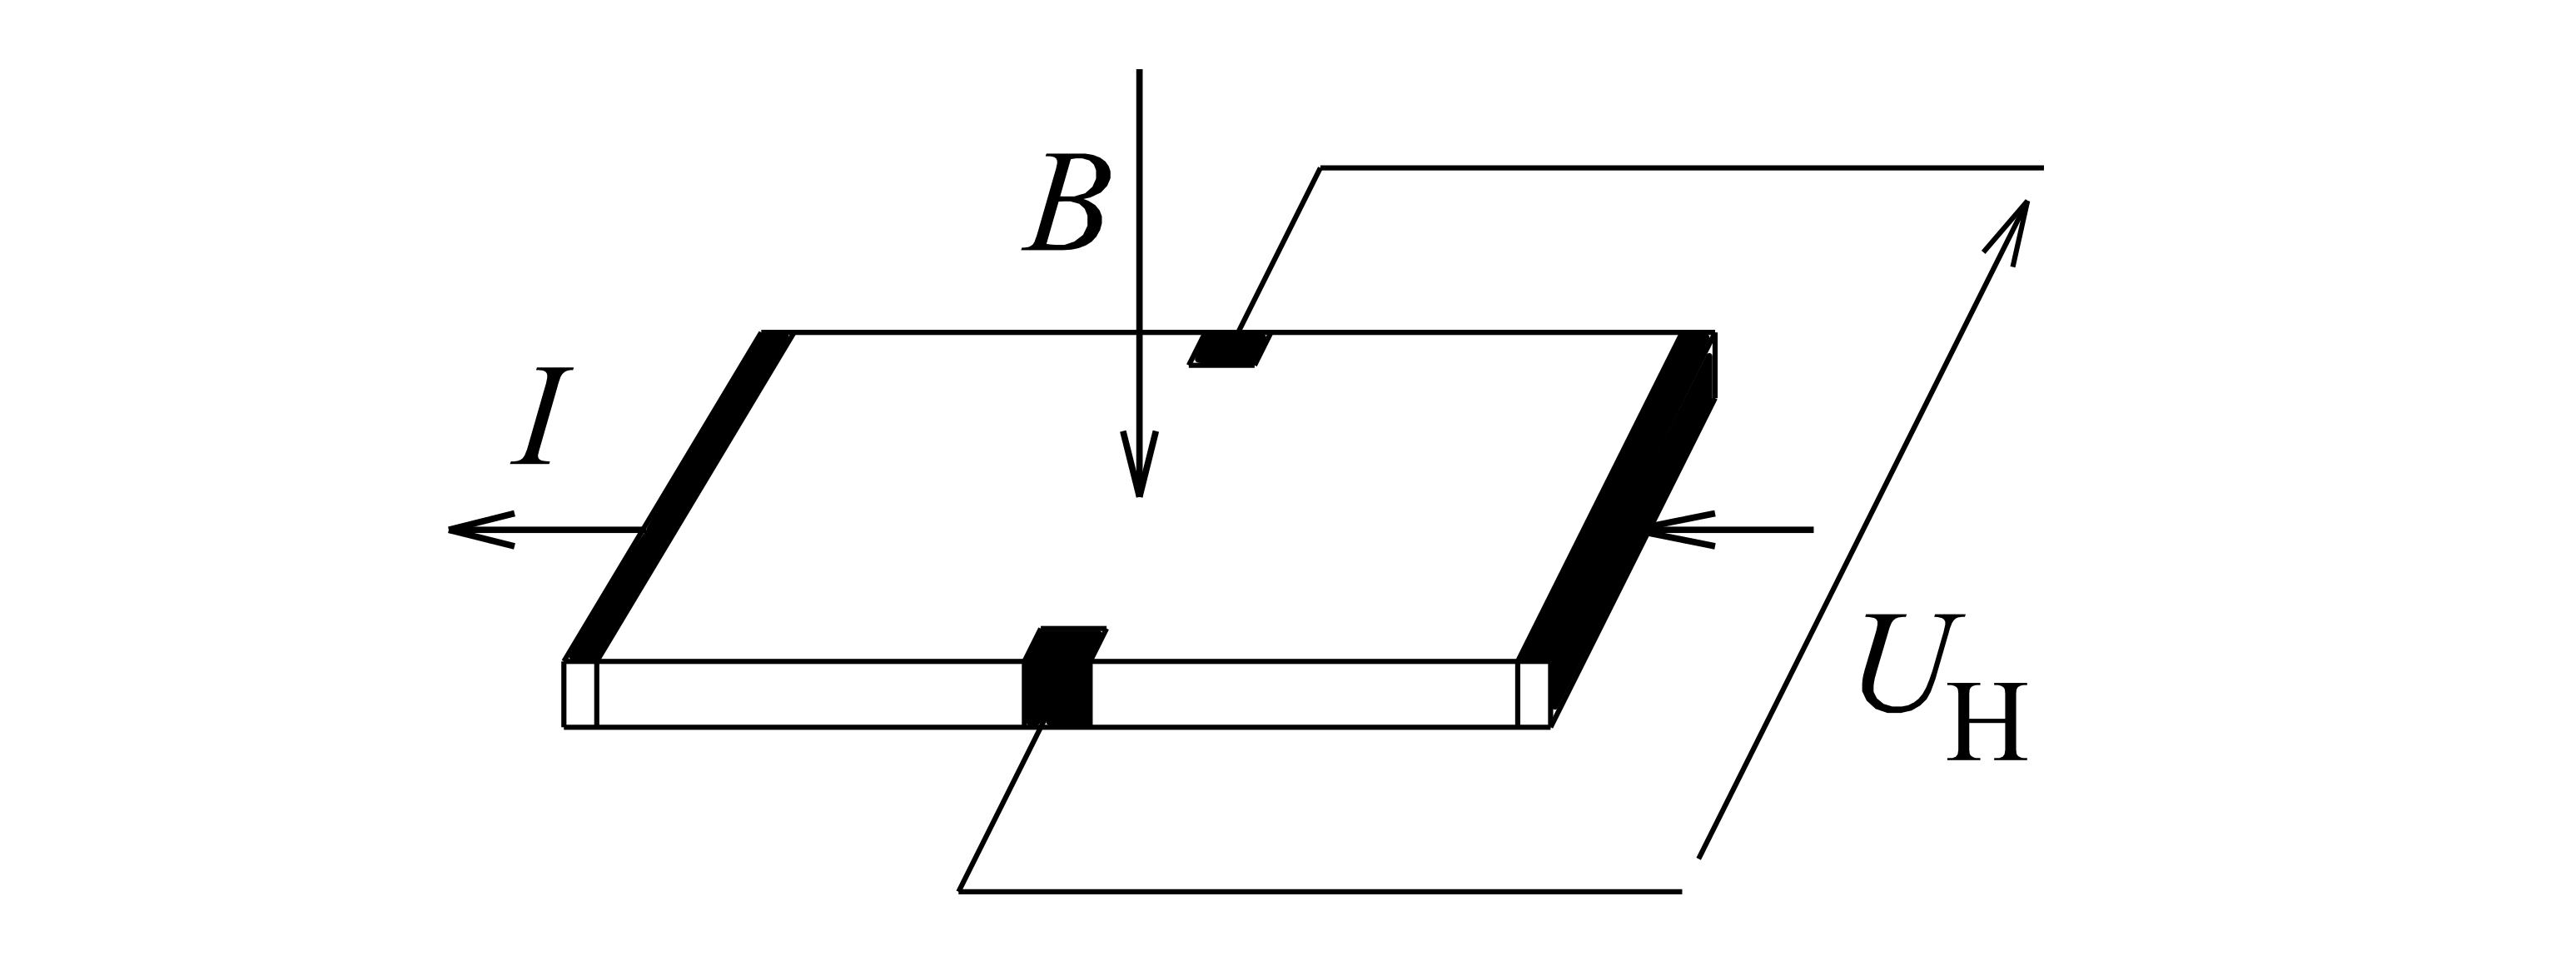
\includegraphics[width=\linewidth]{Halleffekt}
	
	Magnetfeld bewirkt Änderung der Stromrichtung durch Lorentzkraft $\rightarrow$ Spannung quer über den Leiter $\rightarrow$ Elektrisches Feld entsteht $\rightarrow$ Coulombkraft wirkt auf Ladungsträger $\rightarrow$Kräftegleichgewicht:
	
	$\vec{F_c}+\vec{F_L}=\vec{0}$ \hfill daraus \hfill $U_H=\frac{IB}{end}$ 	
	
	\subsection{Magnetisierung}
	
	\note{äusseres Magnetfeld: $\vec{B}_0=\vec{H}\cdot \mu_0$
	
	Durch das Material generiertes Feld: $\vec{B}_M=\vec{M}\cdot\mu_0$
	
	Magnetfeld im Material: $\vec{B}=\vec{B}_0+\vec{B}_M=\vec{H}\cdot \mu_0+\vec{M}\cdot\mu_0=\mu_r\cdot\vec{B}_0$}
	
	Magnetische Suszeptibilität: $\chi_M=\frac{|\vec{B_M}|}{|\vec{B_0}|}=\mu_r-1$
	\vspace{1ex}
	
	\includegraphics[width=\linewidth]{MagSusz}
	
	Magnetische Erregung \hspace{1ex} $\vec{H}=\frac{\vec{B_0}}{\mu_0}$\hfill $[H]=1\frac{A}{m}$
	
	Magnetisierung \hspace{1ex} $\vec{M}=\frac{\vec{B_M}}{\mu_0}$\hfill$|\vec{M}|=M_0$\hfill$[M]=1\frac{A}{m}$
		\subsection{Oberflächenströme}
	
	\mypic{Oberflaechenstrom}
	
	Atomare Kreisströme im Körperinneren heben sich auf \dahe resultierender gebundener Oberflächenstrom:
	
	$\vec{M}=\frac{\vec{m}}{V}=\frac{I\vec{A}}{Ad}=\Vprod{n}{j_A}$
	
	Eine homogen magnetisierte Kugel generiert exakt ein Dipolfeld. Das Dipolmoment
ist gegeben durch die Magnetisierung multipliziert mit dem Kugelvolumen. $\vec{m}=4\pi R^3\vec{M}/3$
	
	\subsection{Atomarer Ursprung des Magnetismus}
	
	
	Atomare Kreisströme: Elektronen umkreisen Kern / Elektronenspin\dahe magnetische Dipole.
	
	
	\begin{tabulary}{\linewidth}{L|L|L}
	Diamagnetismus	&	Paramagnetismus	&	Ferromagnetismus\\
	\hline
	Magnetfeld verstärkt / schwächt atomare Kreisströme (verschieden gerichtete Lorentzkraft)	&	Unkompensierte atomare Kreisströme generieren Dipol	&	Kollektive Ausrichtung von atomaren Dipolen\\
	\hline
	Magnetfeld wird abgeschwächt	&	Magnetfeld wird verstärkt	&	Magnetfeld wird enorm verstärkt\\
	\hline
	Sehr schwach	&	schwach	&	Sehr stark\\
	\hline
	$\mu_r<1$	&	$\mu_r>1$	&	$\mu_r\gg 1$\\	
	\hline
	Unabhängig von der Temperatur	&	Nimmt mit steigender Temperatur zu	&	Verschwindet wenn $T>T_C$\\	
	\hline
	
	\end{tabulary}
	
	\note{Für Paramagnetismus ungepaarte Elektronen nötig \dahe atomare Dipole.
	
	Paramagnetismus analog zu Orientierungspolarisation.
	
	Diamagnetismus analog zu Verschiebungspolarisation.}
	\subsection*{Ferromagnetismus}
	
	\begin{itemize}
	\compaq
	\item
	Sätigungsmagnetisierung: Grösste Magnetisierung des Materials.
	\item
	Remanenzmagnetisierung: Verbleibende Magnetisierung nachdem das äussere Feld $B_0=0$.
	\item
	Koerzitivfeld: Gegengerichtetes Feld das nötig ist umd die Remanenzmagnetisierung aufzuheben. 
	\item
	Curietemperatur: Temperatur bei der ein Material seine ferromagnetischen Eigenschaften verliert.
	\end{itemize}
	 
	\subsection{Magnetische Induktion}
	\begin{itemize}
	\compaq
	\item
	Spannung $\propto$ Fläche der Schleife.
	\item
	Spannung $\propto$ Magnetfeldstärke.
	\item
	Vorzeichen der Spannung wechselt mit Vorzeichen des Magnetfeldes.
	\item
	Spannung $\propto$ Geschwindigkeit der Änderung des Magnetfelds oder der Fläche.
	\end{itemize}
	
	\subsection{Faraday'sches Induktionsgesetz}
	$U=-\frac{d}{dt}\int_A{\Bofr\cdot d\vec{A}=-\vec{d\Phi_M}{dt}}$ \hfill $\Vprod{\nabla}{E}=-\frac{d\vec{B}}{dt}$
	
	\subsection{Lenz'sche Regel}
	
	\small
	Die induzierte Spannung und der induzierte Strom sind so gerichtet, dass sie eine der Ursache entgegengerichtete Wirkung erzielen.
	\normalsize
	
	\subsection{Wirbelströme}
	Wird ein elektrischer Leiter in einem inhomogenen Magnetfeld bewegt, so ändert sich der magnetische Fluss und es werden lokal Ströme induziert.
	
	Wirbelstromverluste nehmen zu mit der:
	\begin{itemize}
	\compaq
	\item
	Geschwindigkeit, mit der der Leiter bewegt wird.
	\item
	Stärke des Magnetfeldes.
	\item
	Dicke des Leiters.
	\item
	Leitfähigkeit des Leiters.
	\end{itemize}
	
	\subsection{Induktivität}
	$L=\frac{\phi_M}{I}=\frac{1}{I}\int_A{\Bofr\cdot d\vec{A}}$ \hfill $[L]=1Henry = 1H=1Tm^2/A$
	
	$I(t) = I_0\frac{t}{T}$ \hfill$U(t) = L\frac{dI}{dt}=\frac{LI_0}{T}$
	
	$E_{magn}=\int_0^T{P(t)dt}=\int_0^T{U(t)I(t)dt}=\int_0^T{\frac{LI_0^2t}{T^2}dt}=\frac{1}{2}LI_0^2$

	für Zylinderspule
	$E_{magn}=\frac{N^2\mu_0 \pi R^2}{2l}I_0^2$
	
	Energiedichte $\omega=\frac{1}{2\mu_0}|\vec{B}|^2$
	
	\subsection{Maxwell'sche Gleichungen}
	
	\renewcommand{\arraystretch}{1.2}
	\small
	\begin{tabulary}{\linewidth}{L|L|L}
	\hline
	1	&	$\vec{\nabla}\Eofr=\frac{\vec{\rho}(\vec{r})}{\epsilon_0}$ & $\oint_A{\Eofr\cdot d\vec{A}=\frac{Q}{\epsilon_0}}$\\
	\hline
	2	&	$\vec{\nabla}\cdot\Bofr=0$ & $\oint_A{\Bofr\cdot d\vec{A}}=0$\\
	\hline
	3&$\Vprod{\nabla}{E}=-\frac{d\Bofr}{dt}$ & $\oint_A{\Eofr\cdot d\vec{L}}=-\frac{d}{dt}\int_A{\Bofr\cdot d \vec{A}} $\\
	\hline
	4&$\Vprod{\nabla}{B}(\vec{r})=\mu_0\vec{j}+\mu_0\epsilon_0\frac{d\Eofr}{dt}$ & $\oint_L{\Bofr\cdot d\vec{L}}=\mu_0I+\mu_0\epsilon_0\frac{d}{dt}\int_A{\Eofr\cdot d\vec{A}}$\\
	\hline
	\end{tabulary}
	\normalsize
	\renewcommand{\arraystretch}{1}
	
	\small
	\begin{enumerate}
	\compaq
	\item
	\textbf{Gesetz von Gauss}: Quellen des elektrischen Feldes sind Ladungen. 
	\item
	\textbf{Gesetz von Gauss für Magnetfelder}: Magnetfeld ist quellenfrei, es gibt keine magnetischen Monopole. 
	\item
	\textbf{Faraday'sches Induktionsgesetz}: Zeitliche Änderung des Magnetfeldes führt zu elektrischem Wirbelfeld. 
	\item
	\textbf{Erweitertes Durchflutungsgesetz}: Elektrische Ströme führen zu einem magnetischen Wirbelfeld. 
	\end{enumerate}
	\normalsize


	\subsubsection{Identität}
	
	$\nabla\times(\nabla\times \vec{E})=\nabla(\nabla\cdot\vec{E})-\nabla^2\vec{E}=-\nabla^2\vec{E}$
	
	\subsection{Maxwell'scher Verschiebungsstrom}
	
	$I_V=\epsilon_0\frac{d\phi_E}{dt}=\epsilon_0\frac{d}{dt}\int_A{\Eofr\cdot d\vec{A}}$
		
	 
	
	\subsection{Elektromagnetisches Nahfeld}
	
	Gilt für nahezu statische Felder und kurze Distanzen. Beiträge der Ladung und des Stromes dominieren.
	
	$\vec{\nabla}\cdot\Eofr=\frac{\rho(\vec{r})}{\epsilon_0}$\hfill$\Vprod{\nabla}{B}(\vec{r})\approx \mu_0\vec{j}$	
	
	 
	
	\subsection{Elektromagnetisches Fernfeld}

	Gilt für hochfrequente Felder und grosse Distanzen. Beiträge der Ableitungen von Elektrischem Feld und Magnetfeld dominieren.
	
	$\Vprod{\nabla}{E}(\vec{r})=-\frac{d\Bofr}{dt}$ \hfill $\Vprod{\nabla}{B}(\vec{r})\approx\mu_0\epsilon_0\frac{d \Eofr}{dt}$

	 
	
	\subsection{Elektromagnetische Wellen}
	
	$c=\frac{1}{\sqrt{\mu_0\epsilon_0}}$ \hfill $c=2.998\cdot 10^8\frac{m}{s}$	
	
	Elektromagnetische Wellen (Licht) sind die Fernwirkung beschleunigter Ladungen.
	
	Das elektrische Feld und das Magnetfeld einer elektromagnetischen Welle stehen senkrecht aufeinander, und sind senkrecht zur Ausbreitungsrichtung.
	
	 
	
	\subsection{Poynting Vektor}
	
	$\vec{S}=\frac{1}{\mu_0}(\vec{E}\times\vec{B})=\vec{E}\times\vec{H}$
	
	Der Betrag des Poynting Vektors entspricht der Leistungsdichte, die durch die elektromagnetische Welle transportiert wird.	

	 
	
	\section{Licht und Wellen}
	
	\subsection{Die eindimensionale Welle}
	
	$\frac{d^2\psi(x,t)}{dt^2}=c^2\frac{d^2\psi(x,t)}{dx^2}$ \hfill $\psi(x,t)=\psi(x-ct,0)$
	
	Wellengleichung der Seilwelle\hfill$\frac{d^2z}{dt^2}=\frac{T}{\mu}\frac{d^2z}{dx^2} = c^2\frac{d^2z}{dx^2}$
	
	mit $c=\sqrt{T/\mu}$ wobei $\mu = m/\Delta x$ und $T=\frac{F}{A}$
	
	 
	
	\subsection{Harmonische Wellen}
	
	$\Psi(x,t)=Re(\Psi_0e^{i(\omega t -kx + \phi)})=\Psi_0cos(\omega t - kx+\phi)$
	
	\begin{tabulary}{\linewidth}{L|L}
	\hline
	Zeitgrössen&Ortsgrössen\\
	\hline
	Kreisfrequenz $\omega$ &Wellenvektor k\\
	\hline
	Frequenz $\nu =\omega / (2\pi)$ &Wellenzahl $\tilde{\nu} =k/(2\pi)$\\
	\hline
	Periodendauer $T = 1/f=2\pi / \omega$&Wellenlänge $\lambda=1/ \tilde{\nu} =2\pi /k$\\
	\hline
	\end{tabulary}

	\vspace{1ex}
	
	$k=\frac{\omega}{c}$ \hfill $c=\lambda \nu$ \hfill $\omega=2\pi\nu$ \hfill $k=\frac{2\pi}{\lambda}$
	
	$k\cdot \omega >0 \rightarrow$ linkslaufend \hfill $k\cdot \omega <0\rightarrow$ rechtslaufend
	\subsection{Superpositionsprinzip}
	
	Eine Summe von Wellenfunktionen sind ebenfalls Lösungen der Wellengleichung.
	
	inverse Fourrier-Transformation:
	
	$\Psi(t,x)=\frac{1}{2\pi}\int_{-\infty}^{\infty}{\psi_0(\omega)e^{i\phi(\omega)}e^{i\omega[t-x/c]}d\omega}$
	
	\subsection{Schwebung}
	
	\footnotesize
	$\psi(\omega)=\psi_0e^{i\omega_1t}+\psi_0e^{i\omega_2t}=\psi_0e^{i\overline{\omega}t}(e^{i\Delta \omega t}+e^{i\Delta\omega t})=\psi_0e^{i\overline{\omega}t}2cos(\Delta\omega t)$
	\normalsize
	
	\fbox{$\omega=2\pi f$}\hfill$\overline{\omega}=\frac{\omega_1+\omega_2}{2}$\hfill$\Delta \omega =\frac{|\omega_1-\omega_2|}{2}$
	
	\textbf{Wichtig:} Frequenz der Einhüllenden ist $\Delta\omega$ aber der Betrag der Schwingung moduliert mit $2\cdot\Delta\omega$!
	
	\importname{Schwebungskreisfrequenz}{$2\cdot\Delta\omega=|\omega_1-\omega_2|$}
	
	 
	
	\subsection{Energie, Leistung, Intensität (Seilwelle)}
	
	$w=\frac{E}{\Delta x}=\frac{1}{2}\mu(\frac{d\psi}{dt})^2=\frac{1}{2}\mu\psi_0^2\omega^2$
	
	$P=\frac{dE}{dt}=\frac{dE}{dx}\frac{dx}{dt}=\frac{E}{\delta x}c=\frac{1}{2}\mu c(\frac{d\psi}{dt})^2=\frac{1}{2}\mu c\psi_0^2\omega^2$
	
	Intensität
	
	1-dimensional: \hspace{3ex} $I=P$\hfill 3-dimensional: \hspace{3ex} $I=\frac{P}{A}$
	
	$I\equiv|\psi^2|=\frac{1}{T}\int_{t=0}^T{|\psi(x,t')|^2dt'}=\frac{1}{2}\psi_0^2$
	
	mittlere Amplitude $\psi_{rms}=\frac{1}{\sqrt{2}}|\psi_0|$ 
	
	\subsection{Impedanz}
	
	\small
	Die Wellenimpedanz ist das Verhältnis von auslenkender Kraft zur Geschwindigkeit der Auslenkung. Sie ist eine Eigenschaft des Mediums und nicht der Welle.\normalsize
	
	$Z=\frac{F_Z}{(\frac{dz}{dt})}\overset{Seilwelle}{\approx}\frac{T}{c}=\sqrt{\mu T}$	
	
	\note{Ein Medium ist durch die Wellenimpedanz und die Wellengeschwindigkeit charakteriesiert.}
	
	\subsection{Dispersion}
	
	$c = c(\omega)=\frac{\omega}{k(\omega)}$
	
	\small
	Eine Welle im dispersiven Medium verändert ihre Form während der Ausbreitung.\normalsize
	
	Phasengeschw.: $\nu_p=\frac{\omega}{k}$\hspace{1ex}\note{(Geschwindigkeit des Wellenmaximums)}
	
	Gruppengeschwindigkeit\hspace{1ex}$\nu_g=\frac{d\omega}{dk}\approx\nu_p+k\frac{d\nu_p}{dk}$ \note{Geschwindigkeit der Einhüllenden des Wellenpakets}
	
	\subsection{Absorption}
	
	$\psi(x,t)=\psi_0e^{-x/\delta_e}e^{i(\omega t-kx+\phi)}$\hfill$\delta_e=c\tau=\frac{2}{\alpha}$
	
	$\delta_e$ charakteristische Abfalldistanz \hfill $\tau$ Abklingzeit 
	
	$\alpha$ Absorptionskoeffizient
	
	$I(x)=I_0e^{-\alpha x}$
	
	Eine Welle mit Absorption zeigt gleichzeitig auch Dispersion, und umgekehrt.
	
	 
	
	\section{Dreidimensionale Wellen}
	
	Ebene Welle \hspace{1ex} $\psi(\vec{x},t)=\psi_0e^{i(\omega t-\vec{k}\cdot\vec{x}+\phi)}$
	
	\subsection*{Dreidimensionale Wellengleichung}
	
	$\frac{d^2\psi(\vec{x},t)}{dt^2}=
	c^2\vec{\nabla}^2\psi(\vec{x},t)=c^2(\frac{d^2}{dx^2}+\frac{d^2}{dy^2}+\frac{d^2}{dz^2})\psi(\vec{x},t)$
	
	Kugelwelle: $\psi(\vec{x},t)=\psi(r,t)=\frac{\psi_0}{\sqrt{4\pi}r}e^{i(\omega t-kr+\phi)}$
	
	 
	
	\subsection*{Transversal, Longitudinal, Rayleigh}
	
	Ist die Amplitude einer Welle eine vektorielle Grösse, so kann die Schwingungsrichtung parallel (Longitudinal) oder senkrecht (Transversal) zur Ausbreitungsrichtung sein.
	
	\mypic{Rayleigh}
	
	\subsection{Wellenausbreitung durch eine Grenzfläche}
	
	Reflexionskoeffizient \hspace{1ex}$r=\frac{\psi_{0,B}}{\psi_{0,A}}=\frac{Z_1-Z_2}{Z_1+Z_2}$\hfill$\Delta\phi=\pi$
	
	Transmissionskoeffizient \hspace{1ex}$t=\frac{\psi_{0,C}}{\psi_{0,A}}=\frac{2Z_1}{Z_1+Z_2}=1+r$
	
	\subsection{Reflexion und Transmission}
	
	B = Reflexion, C = Transmission
	
	$P_B=r^2P_A$\hfill$P_C=P_A-P_B$
	
	Reflexionsgrad $R=\frac{P_B}{P_A}=r^2$
	
	Transmissionsgrad $T=\frac{P_C}{P_A}=1-R$
		
	\vspace{1ex}	
		
	\begin{tabular*}{\linewidth}{l|l|l|l|l}
	\hline
	&$Z_2$&$\psi_{0,B}$&$\psi_{0,C}$&$P$\\
	\hline
	"Wand" &$Z_2\rightarrow\infty$ & $-\psi_{0,A}$ & 0 & $0\%$\\
	"loses Ende"&$Z_2\rightarrow 0$&$\psi_{0,A}$&$2\psi_{0,A}$&$0\%$\\
	Impedanzanpassung&$Z_2 = Z_1$&0&$\psi_{0,A}$&$100\%$\\
	\hline
	\end{tabular*}	
	
	\subsection{Stehende Wellen}
	
	$\psi_A(x,t)=\psi_0e^{i(\omega t -kx+\phi)}$\hfill einfallende Welle
	
	$\psi_b(x,t)=-\psi_0e^{i(\omega t+kx+\phi)}$\hfill refkletierte Welle
	
	Realteil der Superposition: $2\psi_0\sin(kx)\sin(\omega t+\phi)$
	
	\emph{Bei einer stehenden Welle sind die zeitliche und die örtliche Schwingung voneinander separiert.}
	
	\finn
	
	Eine stehende Welle ist eine Überlagerung einer stehenden und einer reflektierten Welle zwischen zwei Mediengrenzen(festes/loses Ende).
	
	Wellenlänge: $\lambda_{gerade}=\frac{2L}{n}$\hfill$\lambda_{ungerade}=\frac{4L}{2n-1}$
	
	Frequenz aus: $f_n=\frac{c}{\lambda_n}$ für n=1 $\rightarrow$ Grundfrequenz.
		
	Gerader Fall für zwei feste (Z=$\infty$) oder zwei lose (Z=0) Enden. Sonst ungerade.
	
	\mypic{StehendeWellen}
	
	\subsection{Akustische Wellen}
	
	Auslenkung aus der Gleichgewichtslage: $s(x,t)=s_0cos(\omega t-kx+\phi)$ 
	
	Schallschnelle: $\nu(x,t)=\frac{ds(x,t)}{dt}=\nu_0sin(\omega t -kx + \phi)$ 
	
	Schalldruck: $p(x,t)=p_0+\delta p_0 sin(\omega t-kx+\phi)$ 
	
	$\nu_0 = -\omega s_0$ = Amplitude der Schallschnelle, $\delta p_0$ = Amplitude des Schalldrucks, $p_0$ = Gleichgewichtsdruck.
	
	$\frac{d^2p}{dt^2}=-K\frac{d}{dt}\frac{d\nu}{dx}=-K\frac{d}{dx}\frac{d\nu}{dt}=\frac{K}{\rho}\frac{d^2p}{dx^2}$
	
	Kompressionsmodul: $K=-V\frac{dp}{dV}$ \hfill $c=\sqrt{\frac{K}{\rho}}$ 
	
	In Gasen: $c=\sqrt{\frac{K}{\rho}}=\sqrt{\frac{\gamma p_0}{\rho}}=\sqrt{\frac{\gamma RT}{M}}$
	
	Akustische Impedanz: $Z=\rho c=\sqrt{K\rho}=\frac{\delta p_0}{\nu_0}$
	
	Schallintensität: $I=\frac{1}{2}\rho c (\frac{ds}{dt})^2=\frac{1}{2}\rho c \nu_0^2=\frac{1}{2}\frac{(\delta p_0)^2}{Z}$\hfill$P=IA$
	
	Schallpegel: $L=10\cdot\log_{10}(\frac{I}{I_0})$ wobei $I_0 = 1\cdot 10^{-12} \frac{W}{m^2}$
	
	\subsection{Akustische Impedanz in Rohren}
	
	$Z_a=\frac{Z}{A}=\frac{\sqrt{K\rho}}{\pi R^2}$
	
	Resonanzfrequenz 2 gleiche Enden: $f_n=\frac{c}{\lambda_n}=\frac{nc}{2L}$
	
	sonst: $f_n=\left(n-\frac{1}{2}\right)\frac{c}{2L}$
	
	\vspace{1ex}	
	
	\begin{tabular*}{\linewidth}{l|l|l|l}
	\hline
	Ende&Z&$\delta_p$&$v$\\
	\hline
	Geschlossen&$Z_a=\infty$&$|\delta_p|=\delta_{p0}$&$v=0$\\
	Offen&$Z_a\approx Z/\lambda^2$&$\delta_p=0$&$|v|=v_0$\\
	\hline	
	\end{tabular*}
	
	\finn	
	
	Intensität halbiert bei Rohrteilung: $\frac{\psi_0}{\sqrt{2}}=\psi_{halbe}$	
		
	\subsection{Dopplereffekt}
	$f_E=f(\frac{c-\nu_E}{c-\nu_S})$ Vom Empfänger wahrgenommene Frequenz.
	
	$sin(\vartheta)=\frac{ct}{v_St}=\frac{c}{\nu_S}$ halber Öffnungswinkel des machschen Kegels.
	
	\subsection{Wellengleichung für elektromagnetische Wellen}
	
	$\frac{d^2\vec{E}}{dt^2}=\frac{1}{\mu_0\epsilon_0}\frac{d^2\vec{E}}{dx^2}$\hfill$\frac{d^2\vec{B}}{dt^2}=\frac{1}{\mu_0\epsilon_0}\frac{d^2\vec{B}}{dx^2}$
	
	$|\vec{B}|=|\vec{E}|/c_0$ \hfill $\vec{E}\perp\vec{B}\perp\vec{S}$ \hfill $\vec{S}=\frac{1}{\mu_0}(\Vprod{E}{B})$
	
	Im Vakuum:
	
	$\vec{E}(x,t)=\vec{E_0}e^{i(\omega t-\vec{k}\vec{x}+\phi)}$\hfill$\vec{B}(x,t)=\vec{B_0}e^{i(\omega t-\vec{k}\vec{x}+\phi)}$
	
	Impedanz: $Z=\frac{E_0}{H_0}=\frac{E_0}{B_0/\mu_0}$
	
	Im Vakuum: $Z_0=\mu_0c_0=\sqrt{\frac{\mu_0}{\epsilon_0}}=\SI{376.37}{\ohm}$
	
	Energiedichte: $\omega=\frac{1}{2}\epsilon_0\frac{E_0^2}{2}+\frac{1}{2\mu_0}\frac{B_0^2}{2}=\frac{1}{2}\epsilon_0E_0^2$
	
	Intensität: $I=\frac{1}{A}\frac{dE}{dt}=\frac{Ac}{A}\frac{\epsilon_0}{2}E_0^2=\frac{1}{2}c\epsilon_0E_0^2$
	
	Sichtbarer Lichtwellenbereich: $\SI{400}{\nano\meter}-\SI{700}{\nano\meter}$
	
	\begin{tabulary}{\linewidth}{L|L}
	\hline
	Zeitgrössen&Ortsgrössen\\
	\hline
	Kreisfrequenz $\omega$ &Wellenvektor k\\
	\hline
	Frequenz $\nu =\omega / (2\pi)$ &Wellenzahl $\tilde{\nu} =k/(2\pi)$\\
	\hline
	Periodendauer $T = 1/f=2\pi / \omega$&Wellenlänge $\lambda=1/ \tilde{\nu} =2\pi /k$\\
	\hline
	\end{tabulary}

	\vspace{1ex}
	
	$k=\frac{\omega}{c}$ \hfill $c=\lambda \nu$ \hfill $\omega=2\pi\nu$ \hfill $k=\frac{2\pi}{\lambda}$
	
	$k\cdot \omega >0 \rightarrow$ linksläufig \hfill $k\cdot \omega <0\rightarrow$ rechtsläufig
	
	\subsection{Elektromagnetische Kugelwelle}
	
	$\vec{E}(r,t)=\frac{A_0}{r}\cdot\sin(kr-\omega t +\phi)=\frac{E_0}{\sqrt{4\pi}r}\sin(kr-\omega t)$
	
	Amplitude an der Stelle r: $E_0=\frac{A_0}{r}$
	
	$I(r)=\frac{1}{2}\epsilon_0 c E_0^2=\frac{1}{2}\epsilon_0 c \left(\frac{A_0}{r}\right)^2$
	
	$P_{tot}=A(r)\cdot I(r)=4\pi r^2 \cdot\frac{1}{2}c\epsilon_0\left(\frac{A_0}{r}\right)^2=2\pi\epsilon_0 c A_0^2$
	
	 
	
	\subsection{Elektromagnetische Wellen in Materie}
	
	In Materialien: Verzögerung und Absorption. Das elektrische Feld führt zu einer Polarisierung des Materials und es baut sich ein Gegenfeld auf.
	
	$c=\frac{1}{\sqrt{\mu\epsilon}}=\frac{1}{\sqrt{\mu_r\mu_0\epsilon_r\epsilon_0}}=\frac{c_0}{\sqrt{\mu_r\epsilon_r}}=\frac{c_0}{n}$\hfill$n=\frac{c_0}{c}$
	
	\note{$\mu_r$ und $\epsilon_r$ nicht konstant bei hohen Frequenzen.}
	
	$\lambda=\frac{\lambda_0}{n}$\hfill$k=\frac{2\pi}{\lambda}=k_0\cdot n$
	
	Optische Distanz: $\sum{d\cdot n}$	
	
	\finn
	
	Impedanz: $Z=\mu c=\sqrt{\frac{\mu}{\epsilon}}=\sqrt{\frac{\mu_r}{\epsilon_r}}Z_0$
	
	Für nichtmagnetische Materialien: $n\approx\sqrt{\epsilon_r}$ \hfill $Z\approx\frac{Z_0}{n}$
	
	für eine senkrecht einfallende elektromagnetische Welle:
	
	$R=(\frac{Z_2-Z_1}{Z_2+Z_1})^2\overset{\mu_1\approx\mu_2}{\approx}(\frac{n_1-n_2}{n_1+n_2})^2$\hfill$T=1-R=\frac{4n_1n_2}{(n_1+n_2)^2}$
	
	\subsection{Lambert-Beer-Gesetz}
		
	Betrachten der Eindringtiefe d von Licht in eine Lösung mit einer zu bestimmenden Konzentration c.
	
	$I(d)=e^{-\alpha d}I_0$
	
	$E=-log_10(e^{-\alpha d})=log_10(e)\alpha d\approx 0.434\alpha d=\epsilon c d$ Lambert-Beer-Gesetz
	
	Hier ist E der Extinktionskoeffizient und $\epsilon$ der molare Extinktionskoeffizient welcher charakteristisch für den gelösten Stoff ist.
	
	 
	
	\subsection{Komplexer Brechungsindex}
	
	\note{Reflexion an einer Metalloberfläche}
	
	$\tilde{k}=k-i\alpha /2$\hfill gedämpfte Welle: $E(x,t)=E_0e^{i(\omega t-\tilde{k}x+\phi)}$
	
	komplexer Brechungsindex: $\tilde{n}=\frac{\tilde{k}}{k_0}=n-i\frac{\alpha}{2k_0}=n-i\kappa$
	
	\note{
	Wobei n und $\kappa$ der reelle und komplexe Anteil des komplexen Brechungsindexes und $k_0=\omega /c_0$ der Wellenvektor im Vakuum sind.}
	
	komplexe Dielektrizitätskonstante: $\tilde{\epsilon_r}=\epsilon_{r,1}+i\epsilon_{r,2}$
	
	$\tilde{n}=\sqrt{\tilde{\epsilon_r}}$
	
	$n=(\frac{1}{2}\sqrt{\epsilon_{r,1}^2+\epsilon_{r,2}^2}-\frac{1}{2}\epsilon_{r,1})^{1/2}$
	
	$\kappa=(\frac{1}{2}\sqrt{\epsilon_{r,1}^2+\epsilon_{r,2}^2}-\frac{1}{2}\epsilon_{r,1})^{1/2}$	
	
	 
	
	\subsection{Reflexionsgrad bei Absorption}
	
	\note{
	Medium 1 ohne Absorption $(\kappa_1=0)$ und Medium 2 mit Absorption $(\kappa_2>0)$.}
	
	$R = |\frac{\tilde{n_1}-\tilde{n_2}}{\tilde{n_1}+\tilde{n_2}}|^2=\frac{(n_1-n_2)^2+\kappa_2^2}{(n_1+n_2)^2+\kappa_2^2}$
	
	\subsubsection{Dielektrizitätskonstante}
	
	\note{\emph{Für sehr tiefe Frequenz verschieben sich die Elektronen im Metall instantan, sodass das elektrische Feld vollständig kompensiert wird.}}
	
	$\epsilon_r(\omega)\rightarrow\infty$ für $\omega\rightarrow 0$	
	
	\note{\emph{Für sehr hohe Frequenz ändert das elektrische Feld so schnell ,dass die Elektronen nicht folgen können.}}
	
	$\epsilon_r(\omega)\rightarrow 0$ für $\omega\rightarrow\infty$	
	
	\subsection{Eindringtiefe}
	
	$\delta_e\approx(\frac{c_0^2}{\omega^2}\frac{2\omega \epsilon_0}{\sigma})^{1/2}=(\frac{2}{\omega\sigma\mu_0})^{1/2}$	 
	
	\subsection{Reflexions- und Brechungsgesetz}
	$n_1\sin(\alpha_1)=n_2\sin(\alpha_2)$\hfill$\alpha_2=\sin^{-1}\left(\frac{n_1}{n_2}\sin(\alpha_1)\right)$
	
	Beim Übergang von einem optisch dünneren zu einem optisch dichteren Medium wird der Strahl zum Lot hin gebrochen.
	
	\note{Prinzip von Huygens: Jeder Punkt einer bestehenden Lichtwelle produziert eine neue Kugelwelle. Alle Kugelwellen summieren sich zu einer neuen Lichtwelle zum späteren Zeitpunkt.}
	
	\note{Prinzip von Fermat: Das Licht nimmt immer den schnellsten Weg, um von Punkt A zu Punkt B zu gelangen.}
	
	\subsection{Totalreflexion}
	
	$\alpha_{1,c}=sin^{-1}(\frac{n_2}{n_1})$
	
	Beim Übergang von einem optisch dichteren in ein optisch dünneres Medium, kann Totalreflexion auftreten.
	
	\subsection{Evaneszenz}
	
	Bei der Totalreflexion wird ein Teil der Welle transmitiert, der dann im Medium exponentiell abfällt. Trotzdem ist der Reflexionsgrad 100\% und es tritt keine Absorption auf. Bei einer Tiefe von $\delta$ ist die Amplitude der Welle auf $1/e$ abgefallen.
	
	Eindringtiefe $\delta = \frac{\lambda_1}{2\pi\sqrt{sin^2\alpha_1-(\frac{n_2}{n_1})^2}}$
	
	Wellenlänge der einfallenden Welle $\lambda_1 = \frac{2\pi}{k_1}$
	
	\subsection{Polarisation}
	
	$\vec{E}(x,t) = \vec{E}_{0,y}e^{i(\omega t-kx+\phi_y)}+\vec{E_{0,z}}e^{i(\omega t-kx+\phi_z)}$
	
	Polarisiertes Licht kann als Superposition von zwei Basiswellen dargestellt werden. Es wird charakterisiert durch die Phasendifferenz $\delta\phi = \phi_y - \phi_z$ und die beiden Amplituden.
	\mypic{ElliptischePolarisation.png}
	
	Lineare Polarisation: $\delta\phi = n\pi \rightarrow \vec{E}$ immer in derselben Ebene.
	
	Zirkularpolarisation: $\delta\phi = (n+\frac{1}{2})\pi \rightarrow \vec{E}$ rotiert in der yz-Ebene und beschreibt einen Kreis.
	
	Rechtsdrehend: $\delta\phi = \pi/2$ \hfill Linksdrehend: $\delta\phi = -\pi/2$
	
	Sonst: Elliptische Polarisation als Superposition von linear und zirkular polarisierten Wellen.
	
	\subsection{Erzeugung linear polarisierten Lichts}
	Absorption: Polarisationsfolie mit parallel verlaufenden Molekülketten. Parallel verlaufendes Feld induziert Ströme. Energie wird absorbiert. Senkrecht dazu Transmissionsachse. Transmittierte Intensität: $I_1=I_0cos^2(45)=\frac{1}{2}I_0$

	Malus'sches Gesetz zur Transmission polarisierten Lichts durch um $\Theta$ gedrehten Polarisator: $I_2 = I_1cos^2(\Theta)$
		
	Reflexion: Mediengrenze mit $n_1$ und $n_2$. Beim Brewster Winkel $tan(\theta_p)=\frac{n_2}{n_1}$ ist die Reflexion rein p-polarisiert.
		
	
	Streuung: Absorption und anschliessende Reflexion an einem einzelnen Teilchen.
	
	Doppelbrechung: (siehe Kapitel Doppelbrechung)
	
	\subsection{Reflexion und Transmission mit Winkel}
	
	horizontal - parallel zur Mediengrenze - s-polarisiert

	vertikal - senkrecht zur Mediengrenze - p-polarisiert
	
	\vspace{1ex}	
	
	$R_s=\left(\frac{cos\alpha_1-\sqrt{(n_2/n_1)^2-sin^2\alpha_1}}{cos\alpha_1+\sqrt{(n_2/n_1)^2-sin^2\alpha_1}}\right)^2$\hfill$Z_{1s,2s}=\frac{Z_0}{n_{1,2}\cos(\alpha_{1,2})}$
	
	$R_p=\left(\frac{\sqrt{(n_2/n_1)^2-sin^2\alpha_1}-(n_2/n_1)^2cos\alpha_1}{\sqrt{(n_2/n_1)^2-sin^2\alpha_1}+(n_2/n_1)^2cos\alpha_1}\right)$\hfill$Z_{1p,2p}=\frac{Z_0\cos(\alpha_{1,2}}{n_{1,2}}$
	
	\note{Wobei 1 für einfallende Welle und 2 für transmittierte Welle.}
	
	\vspace{1ex}	
	
	$R_s+nT_s=1$ \hfill $R_p+nT_p=1$
	
	Brewsterwinkel: Die reflektierte Welle ist komplett s-polarisiert $\rightarrow R_p = 0$.
	
	$\alpha_{1,B}=tan^{-1}(\frac{n_2}{n_1})$
	
	\subsection{Doppelbrechung}
	
	Optisch anisotropes Material \dahe $n,c,\epsilon_r$ hängen von Richtung und Polarisation des eintretenden Lichts ab \dahe Aufspaltung in o-Strahl und ao-Strahl. (p- und s-Anteile erfahren verschiedene $\epsilon_r$!) Richtung in der o und ao gleiche Geschwindigkeit haben \dahe optische Achse.
	
	\note{o - ordentlich, ao - ausserordentlich}
	
	Dann gibt es 3 Fälle:
	
	\begin{itemize}
	\compaq
	\item
	Parallel zur optischen Achse keine Anomalitäten.
	\item
	Senkrecht zur optischen Achse: o und ao sind parallel aber verschieden schnell \dahe Änderung der Polarisation. Bsp.: $\lambda_{\frac{1}{4}}$-Plätchen bewirkt Änderung von Linera zu Zirkular.
	\item
	Doppelbrechung bei allen anderen Winkeln. o-Strahl wird transmittiert und ao-Strahl gebrochen.
	\end{itemize}
	
	\mypic{Doppelbrechung.png}	
	
	\subsection{optische Aktivität}
	
	Hintereinanderreihung von n Polarisatoren mit infinitesimal kleiner Verdrehung von $\beta/n$ bewirkt eine verlustfreihe Drehung eines Lichtstrahls um $\beta$.	
	
	\subsection{Kohärenz}
	
	Zwei Wellen, deren Phasendifferenz an jedem Ort und zu jeder Zeit gleich ist, sind kohärent.
	
	Kohärenzlänge: Distanz nach der die Differenz zwischen Interferenzmaximum- und minimum auf ca. $37\%$ abgefallen ist.
	
	\subsection{Interferenz}
	
	$\Psi_A(x,t) = \Psi_{0,A}e^{i(\omega t-kx+\Psi_A)}$\hfill$\Psi_B(x,t)=\Psi_{0,B}e^{i(\omega t-kx+\Psi_B)}$
	
	$\Psi(x,t)$ ist die Superposition von $\Psi_A$ und $\Psi_B$
	
	\note{
	mit $\bar{\Psi} = \frac{1}{2}(\Psi_{0,A}+\Psi_{0,B})$ und $\Delta\Psi =\frac{1}{2}(\Psi_{0,A}-\Psi_{0,B})$ 
	
	wie auch $\bar{\phi}=\frac{1}{2}(\phi_A+\phi_B)$ und $\Delta\phi=\frac{1}{2}(\phi_A-\phi_B)$}
	
	$\Re(\Psi(x,t))=2\cos(\Delta\phi)\bar{\Psi}\cos(\omega t-kx+\bar{\phi})-2\sin(\Delta\phi)\Delta\phi \sin(\omega t-kx+\bar{\phi})$
	
	für $(\Psi_{0,A}=\Psi_{0,B}=\Psi_0)$: \hfill $\Psi(x,t)=2\cos(\Delta\phi)\Psi_0e^{i(\omega t-kx+\bar{\phi})}$
	
	Intensität: $I = \frac{1}{2}\Psi_0^2 4cos^2(\Delta\phi)$
	
	\begin{itemize}
	\compaq
	\item
	$\Delta\phi=n\pi$ \hfill konstruktive Interferenz
	\item	
	$\Delta\phi=(n+\frac{1}{2})\pi$ \hfill destruktive Interferenz
	\end{itemize}
	
	\subsection{Michelson-Interferometer}
	
	\mypic{MichelsonInterferometer}
	
	Licht wird mit halbdurchlässigem Spiegel aufgeteilt, legt einen unterschiedlichen Weg zurück und wird dann wieder zusammengeführt \dahe Interferenz.
	
	$\Psi_A(x)=\frac{1}{2}\Psi_0e^{-ik(2d+x)}$\hfill Welle via 1. Spiegel
	
	$\Psi_B(x)=\frac{1}{2}\Psi_0e^{-ik(2d+2\Delta d+x)}$\hfill Welle via 2. Spiegel
	
	Überlagerung: \hfill$\frac{1}{2}\Psi_0e^{-ik(2d+x)}(1+e^{-ik2\Delta d})$
	
	$I=I_0\cos^2(k\Delta d)$
	
	Der Abstand zwischen 2 Intensitätsmaxima ist $\lambda/2$.
	
	\subsection{Interferenz an dünnen Filmen}
	
	\mypic{duenneFolie.png}
	
	\note{
	\begin{itemize}
	\compaq
	\item
	\emph{Eintreffende Welle erfährt Phasensprung bei Reflektion.}
	\item
	$k_i$ abhängig vom Medium! $\lambda_{Materie}=\frac{\lambda_0}{n}\quad k_{Materie}=\frac{2\pi n}{\lambda_0}$	
	\end{itemize}
	}
	
	$\Psi_A(x)=-\Psi_0e^{-ik_1x}$
	
	$\Psi_B(x)=-\Psi_0e^{-i(k_1x+k_2 2\Delta d)}$\hfill für $n_3>n_2$
	
	$\Psi_{B'}(x)=-\Psi_0e^{-i(k_1x+k_2 2\Delta d)}$\hfill für $n_3<n_2$
	
	Überlagerung:
	
	$\Psi(x)=-\Psi_0e^{-ik_1x}(1+e^{-ik_2 2\Delta d})$\hfill für $n_3>n_2$
	
	$\Psi(x)=-\Psi_0e^{-ik_1x}(1-e^{-k_2 2\Delta d})$\hfill für $n_3<n_2$
	
	Intensität:
	
	$I=\frac{1}{2}\Psi_0[2+2\cos(k_2 2 \Delta d)]\propto \cos^2(k_2 \Delta d)$\hfill für $n_3>n_2$
	
	$I=\frac{1}{2}\Psi_0[2-2\cos(k_2 2 \Delta d)]\propto \sin^2(k_2 \Delta d)$ \hfill für $n_3<n_2$
	
	Konstruktive Interferenz bei:
	
	$\Delta d = n\frac{\lambda_2}{2}$ \hfill $\Delta d'=(n-\frac{1}{2})\frac{\lambda_2}{2}$
	
	\subsection{Interferenz am Doppelspalt}
	\mypic{InterferenzDoppelspalt.png}	
	
	$L\gg d$ \dahe Strahlen nahezu parallel.
		$I(\alpha)=4I_0\cos^2(\frac{\pi d}{\lambda}sin(\alpha))$
	
	$sin(\alpha_{max})=\pm n\frac{\lambda}{b}$ \hfill $\sin(\alpha_{min})=\pm\frac{2n + 1}{2}\frac{\lambda}{b}$\hfill$n\in \mathbb{N}$
	
	\subsection{Interferenz an N Spalten}
		$I(\alpha)=I_0\frac{\sin^2\left([N\pi d/\lambda]\sin(\alpha)\right)}{\sin^2\left([\pi d/\lambda]\sin(\alpha)\right)}$
	
	 mit $I_0=$ Intensität pro Spalt.
	 
	 Für das zentrale Maximum: $I(\alpha)\approx I_0N^2$
	
	\subsection{Beugung am Spalt}
	Streuung einer ebenen Welle am Spalt mit Breite $b$.
	
	$I(\alpha)=I_{tot}\frac{\sin^2\left([b\pi/\lambda]\sin(\alpha)\right)}{\left([b\pi/\lambda]\sin(\alpha)\right)^2}$
	
	$sin(\alpha_{max})=\pm\frac{2n+1}{2}\frac{\lambda}{b}$\hfill	$sin(\alpha_{min})=\pm n\frac{\lambda}{b}$	\hfill $n\in\mathbb{N}$
	
	\subsection{Beugung am Mehrfachspalt}
	
	$I(\alpha)=I_{tot}\underbrace{\frac{\sin^2\left([b\pi/\lambda]\sin(\alpha)\right)}{\left([b\pi/\lambda]\sin(\alpha)\right)}}_{Beugung}\underbrace{\frac{\sin^2\left([N\pi d/\lambda]\sin(\alpha)\right)}{\sin^2\left([\pi d/\lambda]\sin(\alpha)\right)}}_{Interferenz}$	
	
	\subsection{Beugung an einer allgemeinen Blende}
	Allgemeine Blende bei $x=0$ mit Elementarwellen auf der Blendenfläche an den Stellen $\vec{r}'=(0,y',z')$ mit Schirm in grossem Abstand x=L.
	
	\finn	
	
	$\Psi(\vec{r})=\int_A{\frac{\Psi_0}{\sqrt{4\pi}|\vec{r}-\vec{r}'|}e^{ik|\vec{r}-\vec{r}'|}dx'dy'}$ \hfill Integral über die Fläche der Blende $A$.
	
	Vereinfacht: $\Psi(y,z)=\frac{\Psi_0}{\sqrt{4\pi}R}e^{ikR}\int_A{e^{i(k_yy'+k_zz')}dy'dz'}$
	
	\note{$R=\sqrt{L^2+y^2+z^2}$ und $k_y = ky/R$}
	
	$I(y,z) = \frac{I_{tot}}{4\pi R^2}|\int_A{dy'dz'e^{i(k_yy'+k_zz')}}|$
	
	\dahe Das Beugungsbild ist durch die räumliche Fouriertransformation der Blende gegeben. Daher kann man aus dem Beugungsbild Rückschlüsse auf die Form der Blende ziehen.	
	
	\subsection{Beugung an der Lochblende}
	
	$I(\alpha)=I_{tot}(\frac{2J_1([2\pi R/\lambda]sin(\alpha))}{[2\pi R/\lambda]sin(\alpha)})^2$ 
	
	\note{mit $R = D/2$ Radius des Lochs}
	
	$J_1(x)=\frac{1}{\pi}\int_0^\pi{cos(n\phi-xsin\phi)d\phi}$
	
	$sin(\alpha_{min})=n\frac{\lambda}{2R}$ \hfill mit $n=1.22,2.23,3.24,...$
	
	\subsection{Auflösungsvermögen}
	
	$sin(\alpha_{min})=1.22\frac{\lambda}{D}\overset{\lambda\ll D}{\approx}\alpha_{min}\approx \frac{z}{L}$ \hfill Rayleigh-Kriterium
	
	\section{Welle-Teilchen Dualismus}
	
	$h = 6.626\cdot 10^{-34}$ $Js=4.136$ $eV/Hz$
		
	\subsection{Das Photon}

	Die Amplitude der elektromagnetischen Welle kann nur diskrete Werte annehmen.

	Das Photon: Lichtquant, hat Energie und Impuls, verhält sich also wie ein Teilchen.
	
	Die kinetische Energie des Photons hängt nur vom der Frequenz und nicht von der Intensität ab.

	Lichtenergie eines Photons mit Frequenz $\nu$: $E = h\nu$
	
	\subsubsection{Photoelektrischer Effekt}
	
	Elektronen treten unter Lichteinfall aus der Metallplatte aus. Durch erhöhung des Feldes kann die kinetische Energie der Elektronen gemessen werden.
	
	$E_{kin}=\frac{1}{2}m_ev_e^2=h\nu-W_{aus}=h\nu-e\phi_{aus}$
	
	\mypic{PhotoelektrischerEffekt.png}
	
	 
	
	\subsubsection{Strahlungsdruck / Impuls}
	
	$P=\frac{I}{c}$\hfill$I=\frac{P}{A}=\frac{E\dot{N}}{A}$\hfill$p = \frac{E}{c}=\frac{h}{\lambda}$\hfill$F=\frac{\Delta p}{\Delta t}=\dot{N} p$
	
	\notelist{
	\item
	E = Energie pro Photon
	\item
	A = Fläche
	\item
	$\dot{N}$ = Anzahl Photonen	pro Sekunde
	\item
	F bei Reflektion doppelt so gross wie bei Absorption
	}	
	
	Relativitische Energie eines Teilchens: 
	
	$E = \sqrt{p^2c^2+(mc^2)^2}$\hfill$(m\rightarrow 0)\Rightarrow E = pc$
	
	 
	
	\subsection{Compton-Effekt}
	
	\mypic{ComptonEffekt.png}
	
	$p=\frac{h}{\lambda}$\hfill$E=pc=\frac{hc}{\lambda}$
	
	$E_{kin,2}=c(p_1-p_2)$\hfill$\cos^{-1}(1-\frac{\Delta\lambda}{\lambda_{Compton}})$
	
	Es gilt Impulserhaltung: $\vec{p_1}=\vec{p_2}+\vec{p_e}$
	
	$\rightarrow p_e^2=p_1^2+p_2^2-2p_1p_2\cos(\theta)$
	
	und Energieerhaltung: $E_1+E_{e,1}=E_2+E_{e,2}$
	
	$\rightarrow p_1c+m_ec^2=p_2c+\sqrt(p_e^2c^2+(m_ec^2)^2) $
	
	$\rightarrow p_1c+m_ec^2=p_2c+\sqrt(p_e^2c^2+(m_ec^2)^2)$
	
	$ \rightarrow p_e^2=p_1^2-2p_1p_2+p_2^2+2(p_1-p_2)m_ec$
	
	aus Impuls und Energie:
	
	$\frac{p_1-p_2}{p_1p_2}=\frac{1}{m_ec}(1-\cos(\theta))$\hfill$\frac{E_2}{E_1}=\frac{\lambda_1}{\lambda_2}=\frac{1}{1+E_1/(m_ec^2)\cdot (1-cos(\theta))}$
	
	\subsubsection{Spezialfall $\Theta=180^\circ$}
	
	\important{$p_1=\frac{E_{kin,e}\pm\sqrt{E_{kin,e}^2}+2c^2m_eE_{kin,e}}{2c}$}
	
	\subsubsection{Compton-Wellenlänge}
	
	$\lambda_{Compton}=\frac{h}{m_ec}$\hfill$\lambda_2-\lambda_1=\lambda_{Compton}(1-cos(\theta))$
	
	für den Fall das $\theta = 90^{\circ}:\quad\frac{E_2}{E_1}=\frac{1}{1+E_1/(m_ec^2)}$
	
	\section{Materialwellen (QM)}
	
	De Broglie Frequenz: $\nu=\frac{E_{kin}}{h}$
	
	De Broglie Wellenlänge: $\lambda=\frac{h}{p}=\frac{h}{\sqrt{2mE_{kin}}}=\frac{h}{m v}$
	
	\subsection*{Wahrscheinlichkeitsdichte}
	
	$P(x)=|\psi(x)|^2$\hfill$\intinf{P(x)dx}=\intinf{|\psi(x)|^2dx}=1$
	
	$\expval{a}=\intinf{\psi^*(x)a(x)\psi(x)dx}$\hfill$\expval{x}=\intinf{xP(x)dx}$
	
	$\sigma_x=\sqrt{\expval{x^2}-\expval{x}^2}$
	
	$\Psi(x,t)=\psi\cdot e^{i\Theta}\rightarrow |\Psi|^2=e^{-i\Theta}\psi^\ast\cdot e^{i\Theta}\psi=\psi^\ast\psi=|\psi|^2$	
	
	\subsection*{Energie und Impuls}
	
	$\hat{E}=i\hbar\frac{\partial}{\partial t}$\hfill$\hat{p}=-i\hbar\frac{\partial}{\partial x}$
	
	\subsection*{Heisenberg'sche Unschärferelation}

	$\sigma_x\sigma_p\geq\frac{\hbar}{2}\qquad\sigma_E\sigma_t\geq\frac{\hbar}{2}\qquad\sigma_x=c\sigma t\qquad\sigma_p=\sigma_E/c$
	
	\subsubsection{Impulsunschärfe $\leftrightarrow$ Wellenlängenunschärfe}
	
	$\lambda = \lambda + \Delta\lambda$\hfill$p=p+\Delta p$
	
	$p+\Delta p=\frac{h}{\lambda+\Delta\lambda}\rightarrow\Delta p=\frac{h}{\lambda+\Delta\lambda}-\frac{h}{\lambda}=h\frac{\lambda-\lambda+\Delta\lambda}{\lambda(\lambda+\Delta\lambda)}=p\frac{\Delta\lambda}{\lambda}$
	
	\subsection*{Schrödingergleichung}
	
	\fbox{$-\frac{\hbar^2}{2m}\frac{\partial^2 \psi(x,t)}{\partial x^2}+E_{pot}(x,t)\psi(x,t)=i\hbar\frac{\partial \psi(x,t)}{\partial t}$}
	
	\finn
	
	$-\frac{\hbar^2}{2m}\frac{\partial^2\psi(x)}{\partial x^2}+E_{pot}(x)\psi(x)=E\psi(x)$
	
	\finn	
	
	3D: \fbox{$-\frac{\hbar}{2m}(\frac{\partial^2}{\partial x^2}+\frac{\partial^2}{\partial y^2}+\frac{\partial^2}{\partial z^2})\psi+E_{pot}\psi=E\psi$}
	
	\subsection*{Das Teilchen im Kasten}
	
	$E_{pot}=\begin{cases}
	0&\text{falls}\quad 0<x<L\\
	\infty% \text{sonst}	
	\end{cases}$
	
	Schrödingergleichung im Kasten: $-\frac{\hbar^2}{2m}\frac{\partial^2\psi(x)}{\partial x^2}=E\psi(x)$
	
	\finn
	
	Ansatz: $\psi(x)=\psi_{0,A}\sin(kx)+\psi_{0,B}\cos(kx)$ \hfill$E=\frac{\hbar^2 k^2}{2m}$
	
	\finn	
	
	Randbedingungen: $\psi(0)=0\qquad\psi(L)=0$
	
	$\Rightarrow \psi_{0,B}=0\Longrightarrow k_n=\frac{\pi}{L}n$
	
	\finn
	
	Normierung führt zu: $\psi_{0,A}=\sqrt{\frac{2}{L}}$
	
	
	\begin{center}
	\fbox{$\psi_n(x)=\sqrt{\frac{2}{L}}\sin(\frac{\pi n x}{L})$}
	\vspace{1ex}
	\fbox{$E_n=\frac{\hbar^2k_n^2}{2m}=\frac{h^2n^2}{8mL^2}\qquad n=1,2,3,...$}
	\end{center}
	
	Energie im Grundzustand $E_1=\frac{h^2}{8mL^2}$
	\begin{center}
	\emph{Ein gebundenes Teilchen kann sich nur in bestimmten Zuständen mit einer bestimmten Energie befinden.}
	\end{center}

	\subsection*{Harmonischer Oszillator}
	
	$E=E_{kin}+E_{pot}=\frac{p^2}{2m}+\frac{m\omega^2}{2}x^2$
	
	$\Psi=A_0e^{-ax^2}$\hfill$a=\frac{m\omega_0}{2\hbar}$\hfill$A_0^2=\sqrt{\frac{2a}{\pi}}$
	
	$\expval{E_{pot}}=\frac{1}{2}m\omega^2\expval{x^2}$\hfill$\expval{x^2}=\frac{\hbar}{2m\omega_0}$
	
	\finn
	
	Mittlere kinetische Energie entspricht mittlerer potentieller Energie: $\expval{E_{pot}}=\expval{E_{kin}}$
	
	\finn
	
	$\expval{E_{kin}=\frac{\expval{p^2}}{2m}}$\hfill$\expval{p^2}=\frac{1}{2}\hbar m \omega_0$
	
	Federkonstante $k_f=\mu\omega_0^2$\hfill$\mu=\frac{m_H^2}{2m_H}$\hfill$\Delta E =\hbar\omega_0$

	\section{Atomphysik}
	
	\subsection{Bohr'sches Atommodel}	
	
	Schwerer Atomkern, der von leichten Elektronen umkreist wird.
	
	Energie eines Elektrons auf seiner Kreisbahn: $E = -\frac{Ze^2}{8\pi\epsilon_0r}$
	
	\note{Radius abhängig von Zustand des Elektrons: $r_n=a_0n^2$}
	
	\subsection*{Bohr'sche Postulate}
	
	\begin{enumerate}
	\item
	Die Elektronen können sich nur in bestimmten Umlaufbahnen aufhalten. Die Länge einer Umlaufban muss genau einem Vielfachen der de Broglie Wellenlänge entsprechen.
	\item
	Die Umlaufbewegung erfolgt ohne Energieverlust (strahlungsfrei).
	\item
	Wechselt das Elektron zwischen zwei Bahnen, so wird die Energie von aussen aufgenommen oder nach aussen abgegeben. Dabei gilt Energierhaltung.
	\end{enumerate}
	
	De Broglie: $\lambda = \frac{h}{p}=\frac{h}{\sqrt{2mE_{kin}}}$
	
	Elektronenradien: $r_n=\frac{n}{2\pi}\lambda$
	
	Elektronendrehimpuls: $L_n=n\hbar$
	
	\subsection{Energieniveaus von Einelektronatomen}
	
	Bohrradius: $a_0=\frac{4\pi \epsilon_0\hbar^2}{e^2m_e}=\SI{0.0529}{\nano\meter}\qquad r_n=\frac{n^2}{Z}a_0$
	
	$E_1 = -\frac{m_ee^4}{32\pi^2\epsilon_0^2\hbar^2}=-hcR_\infty=\SI{-13.6}{\electronvolt}\qquad E_n=\frac{Z^2}{n^2}E_1$
	
	\note{(Kernladungszahl Z = 1)}
	
	\finn
	
	$E_m-E_n=-hcR_{\infty}Z^2\left(\frac{1}{m^2}-\frac{1}{n^2}\right)$\hfill \hlcyan{für IE: $m=\infty$}
	
	$R_{\infty}=\frac{me^4}{8\epsilon_0^2h^3c}=\SI{10.973731e6}{\per\meter}$
	
	\mypic{Elektronenuebergaenge}
	
	\subsection{Wellengleichung des Einelektronenatoms}
	
	Schrödingergleichung in 3D, polarkoordinaten liefert für das Coulombpotential $E_{pot}=-\frac{Z_e^2}{4\pi\epsilon_0r}$ des positiv geladenen Atomkerns die Lösungen:
	
	\footnotesize	
	$\psi_{nlm_l}(r,\theta,\psi)=\underbrace{\sqrt{(\frac{2}{na_0})^3\frac{(n-l-1)!}{2n(n+l)!}}}_{Normierung}\cdot\underbrace{e^{-\rho/2}\rho^lL_{n-l-1}^{2l+1}(\rho)}_{radial}\cdot\underbrace{Y_l^{m_l}(\theta,\psi}_{winkelabh.}$
	\normalsize
	
	\finn	
	
	mit: $\rho=\frac{2Zr}{na_0}$ und \fbox{$n,l,m_l$ (Quantenzahlen)}
	
	\finn
	
	$E_{n,l,m_l}=E_n=\frac{Z^2}{n^2}E_1$
	
	\finn	
		
	\footnotesize
	\begin{tabulary}{\linewidth}{lLLL}
	&Radiale Quantenzahl&Drehimpulsquantenzahl&Magnetische Quantenzahl\\
	\hline
	Symbol&$n$&$l$&$m_l$\\
	\hline
	Koord.&$r$&$\theta$&$\phi$\\
	\hline
	Grösse&$E_n=E_1Z^2/n^2$&$L=\sqrt{l(l+1)}\hbar$&$L_z=m_l\hbar$\\
	\hline
	&Kn+1&Kn-Eb&Lage der Kn-Eb
	\end{tabulary}
	\normalsize
	
	\subsubsection{Radiale Quantenzahl}
	
	Bestimmt die Wahrscheinlichkeit, das Elektron in einem bestimmten Abstand vom Kern vorzufinden. Anzahl der Knoten in der Wellenfunktion $= n-1$.
	
	\subsubsection{Magnetische Quantenzahl}

	Gibt die Komponente des Drehimpulses entlang einer Richtung (z.b. z) an. Kreisbewegung des Elektrons \dahe magnetischer Dipol mit $\vec{m}=-\frac{e}{2m_e}\vec{L}$ und $\vec{m_z}=-\mu_Bm_l$.
	
	$\mu_B=\SI{9.274e24}{\joule\per\tesla}$
	
	\subsection{Spin}
	
	$S=\sqrt{\frac{3}{4}}\hbar\qquad S_z=m_s\hbar=\pm\frac{1}{2}\hbar$
	
	magnetischer Dipol des Elektrons in z: $m_z=-g_e\mu_Bm_s$
	
	$g_e\approx 2.002$
	
	\subsection{Pauliprinzip}
	
	\emph{Zwei identische Teilchen mit halbzahligem Spin s können nie in allen Quantenzahlen übereinstimmen.}
	
	\dahe Es fallen nicht alle Elektronen in den Grunzustand wie man aus dem Energieminimumprizip annehmen würde.
	
	\section{Absorption und Emission}
	
	\subsection{Atomspektren}
	
	\hbox{$E_2-E_1=E_p=h\nu=\frac{hc}{\lambda}$}
	
	Rydbergformel für Einelektronatome:\fbox{$\frac{1}{\lambda}=R_HZ^2(\frac{1}{n_2^2}-\frac{1}{n_1^2})$} für Wasserstoffähnliche Atome
	
	$R_H=\frac{E_1}{hc}=\SI{1.10e7}{\per\meter}$
	
	 
	
	\subsection{Einstein'sche Koeffizienten}
	
	\begin{itemize}
	\compaq
	\item Absorption:
	Übergang eines Elektrons zu höherer Energie.
	\item Spontane Emission:
	Elektron emittiert spontan ein Photon geht über zu tieferer Energie.
	\item Stimulierte Emission:
	Einfallendes Photon induziert Übergang des Elektrons zu tieferer Energie und löst ein weiteres Photon.
	\end{itemize}
	
	Anzahl Atome N:
	$\begin{cases}
	N_1$: Anzahl Atome auf $E_1\\
	N_2$: Anzahl Atome auf $E_2
	\end{cases}$
	
	\begin{align*}
	\frac{\partial N_1}{\partial t} & = -\rho(\nu)B_{12}N_1+\rho(\nu)B_{21}N_2+A_{21}N_2\\
	\frac{\partial N_2}{\partial t} & = +\underbrace{\rho(\nu)B_{12}N_1}_{Absorption}-\underbrace{\rho(\nu)B_{21}N_2}_{stim. Emission}-\underbrace{A_{21}N_2}_{spont. Emission}
	\end{align*}
	
	\important{$N_2=N_1\frac{B_{21}\rho(E)}{B_{21}\rho(E)+A_{21}}\Rightarrow N_2<N_1$\dahe No LASER!}	
	
	$B_{21}=B_{12}\qquad [B_{12}]=\si{\per\joule\meter\cubed\per\second}\qquad [A_{21}]=\si{\per\second}$
	
	$\rho(\nu)=\frac{1}{2}\epsilon|\vec{E}(\nu)|^2\qquad \rho(\nu)\propto N_p$ 
	
	\note{wobei $\vec{E}(\nu)$ Amplitude des Elektrischen Felds mit Frequenz $\nu$ und $N_p$ Anzahl Photonen.}
	
	 

	\subsection{Grundprinzip des Lasers}
	
	Auffüllen des oberen Energieniveaus mit Elektronen und anschliessende stimulierte Emission führt zu Kettenreaktion. (Laserblitz)
	
	Besetzungsinversion: Das obere Energieniveau muss mehr Elektronen enthalten als das Untere. \textbf{Nur für 3 oder mehr Niveaus realisierbar}, für 2-Niveau-System $N_2\leq\frac{1}{2}$\dahe keine Kettenreaktion.
	
	Für den \textbf{Dreiniveaulaser}:
	
	\begin{align*}
	\frac{\partial N_1}{\partial t}&=+\Gamma_BN_p(N_2-N_1)+\Gamma_AN_2-R_pN_1\\
	\frac{\partial N_2}{\partial t}&=-\Gamma_BN_p(N_2-N_1)-\Gamma_AN_2+\Gamma_{32}N_3\\
	\frac{\partial N_3}{\partial t}&=R_pN_1-\Gamma_{32}N_3
	\end{align*}
	
	\mypic{3NiveauLaser}
	
	Gleichgewicht: $\frac{\partial N_1}{\partial t}=\frac{\partial N_2}{\partial t}=\frac{\partial N_3}{\partial t}=0$
	
	$\Gamma_{32}\gg R_p\Rightarrow N_3 \approx 0\qquad \Delta N = N_2-N_1$
	
	\finn	
	
	\dahe $\frac{\partial \Delta N}{\partial t}=-2\Gamma_BN_p\Delta N-\Gamma_A(N+\Delta N)+R_p(N-\Delta N)=0$
	
	\finn	
	
	\dahe \fbox{$\frac{\Delta N}{N}=\frac{R_p-\Gamma_A}{2\Gamma_BN_p+R_p+\Gamma_A}>0$} \dahe Inversion!
	
	\subsubsection{Photonenverlustrate}
	
	$\frac{\partial N_P}{\partial t}=\Gamma_B(N_2-N_1)N_P+\Gamma_AN_2-R_{leak}N_P$
	
	$R_{leak}=\frac{c}{2nL}(1-R_2)$\hfill$t_0=\frac{1}{R_{leak}}$
	
	$\Gamma_B=\frac{1}{M\Delta\nu\tau}\qquad M=V8\pi\frac{\nu^2}{\frac{c}{n}^3}$
	
	\importname{Besetzungsinversion}{$N_2-N_1>\frac{1}{\Gamma_B\cdot t_0}$}
	
	\notelist{
	\item L = Länge zwischen Spiegeln
	\item n = Brechungsindex des Lasermediums
	\item $R_2$ = Reflexionsgrad des Austrittsspiegels	
	\item $t_0$ = Photonenlebensdauer
	\item $\tau$ = Lebensdauer des Elektrons im Niveau 2
	}
	
	\subsubsection{Eigenschaften}
	
	\begin{itemize}
	\compaq
	\item \textbf{Kohärenz:}
	Alle Photonen haben dieselbe Wellenlänge, Frequenz und Phase.
	\item \textbf{Polarisation:}
	Alle Photonen haben dieselbe Polarisation	
	
	\end{itemize}	
	
	\subsubsection{Aufbau}
	
	\mypic{LaserAufbau}
	
	\begin{itemize}
	\compaq
	\item \textbf{Pumpmechanismus}
	Liefert die Energie \dahe hebt Elektronen im Lasermedium auf ein höheres Energieniveau. (Blitzlichtlampe, chemische Reaktion, elektrische Energie, andere Laser)
	\item \textbf{Lasermedium}
	Im Lasermedium findet die stimulierte Emission statt. Kriterien sind: effiziente stimulierte Emission, schwache spontane Emission und die gewünschte Wellenlänge des Lasers.
	\item \textbf{Laserhohlraum}
	Ein resonanter Hohlraum reflektiert das Licht kontinuierlich, so dass die stimulierte Emission verstärkt wird. ($N_p$ steigt an) Optimalerweise ist die Länge des Hohlraums ein vielfaches der halben Wellenlänge des Laserlichts \dahe stehende Wellen.	
	\end{itemize}
	
	\begin{tabulary}{0.93\linewidth}{p{0.21\linewidth}L}
	Gaslaser&Zwei Gase: Eines dient als Pumpmedium, das andere als Lasermedium.\\
	Feststofflaser& Ähnlich wie Gaslaser, aber das Pump- und Lasermedium sind Feststoffe.\\
	Dye-Laser&Organische Moleküle als Pump- und Lasermedium.\\
	Faserlaser&Feststofflaser in einer Glasfaser, Faser als Lasercavity.\\
	Chemische Laser&Populationsinversion wird durch kontinuerliche chemische Reaktionen aufrechterhalten.
	\end{tabulary}
	\begin{tabulary}{0.93\linewidth}{p{0.21\linewidth}L}
	Halbleiterlaser&Halbleiterdiode, in einer Lasercavity eingebettet. Diode wird elektrisch angeregt.\\
	Free Electron Laser (FEL)&Freie Elektronen,auf relativitische Energien beschleunigt, als Pump- und Lasermedium.\\
	MASER&Analog zur Laseremission im Mikrowellenbereich.
	\end{tabulary}
	
	\section{Festkörperphysik}
	
	\subsection{Bändermodell}
	
	Was passiert wenn man Atome einander annähert?
	
	\begin{itemize}
	\compaq
	\item Reihenfolge der Energieneveaus bleibt erhalten, da sie für einzelne Atome weit aus einander liegen.
	\item Bei Annäherung von 2 Atomen geringfügige Verscheibung der ursprünglich identischen zu zwei Neuen. Leicht höher/tiefer als Orgninalniveaus. 
	\item Bei Annäherung von N Atomen spaltet sich ein gegebenes Niveau zu N leicht unterschiedlichen auf \dahe Energieband.
	\item Je höher Orginalniveau desto breiter enstehendes Energieband.
	\end{itemize}
	
	\mypic{Energieband}
	
	\subsubsection{Gebundene und freie Elektronen}
	
	\begin{itemize}
	\compaq
	\item Tiefere Energiebänder haben eine geringe Aufspaltung, sind fast vollständig am Atom lokalisiert.
	\item Höhere Energiebänder sind stark aufgespalten und die Elektronen können sich fast frei über den Festkörper bewegen. Die Kernladung wird durch die gebundenen Elektronen abgeschirmt.
	\end{itemize}
	
	\subsection{Fermienergie}
	
	\emph{Die Fermienergie $E_F$ ist die Energie des höchsten besetzten Energiniveaus, relativ zum tiefsten besetzen Niveau $E_1$}

	\finn
	
	Hat ein Festkörper $M$ Elektronen sind $M/2$ Niveaus besetzt, da jedes Niveau nach Pauli 2 Elektronen aufnehmen kann.
	
	\subsubsection{Fermienergie 1D/2D/3D Potentialbrunnen}
	
	\begin{tabular}{l|l|l}
	1D&2D&3D\\
	$E_{n_x}=\frac{\hbar^2k_x^2}{2m}$&$E_{n_{x,y}}=\frac{\hbar^2(k_x^2+k_y^2)}{2m}$&$E_{n_{x,y,z}}=\frac{\hbar^2(k_x^2+k_y^2+k_z^2)}{2m}$\\
	$k_F=k_x$&$k_F=\sqrt{k_x^2+k_y^2}$&$k_F=\sqrt{k_x^2+k_y^2+k_z^2}$\\
	$V_1=\frac{\pi}{L_x}$&$V_2=\frac{\pi^2}{L_xL_y}$&$V_3=\frac{\pi^3}{L_xL_yL_z}$\\
	$V_{tot,1}=k_F$&$V_{tot,2}=\frac{1}{4}k_F^2\pi$&$V_{tot,3}=\frac{1}{8}\cdot\frac{4}{3}k_F^3\pi$\\
	\multicolumn{3}{c}{\vspace{-1ex}}\\
	\multicolumn{3}{c}{$k=\frac{N\pi}{L}$\hfill$ n=\frac{M}{L^{(D)}}$\hfill$N=\frac{M}{2}$}\\
	\multicolumn{3}{c}{$V_{tot,D}=V_DN=V_D\frac{M}{2}$\hfill$L_i=L$\hfill$\rightarrow E_F(k_F)=?$}\\
	\multicolumn{3}{c}{$E_F=\frac{\hbar^2 k_F^2}{2m}$}\\
	\multicolumn{3}{c}{\vspace{-1ex}}\\
	$E_{F,1}=\frac{h^2 n^2}{32m_e}$&$E_{F,2}=\frac{h^2n}{4\pi m_e}$&$E_{F,3}=\frac{h^2}{8m_e}\cdot\frac{3n}{\pi}^{2/3}$
	\end{tabular}
	
	\subsubsection{Zustandsdichte}
	
	$g(E)=\frac{\partial n(E)}{\partial E}$\hfill$n_E\propto g(E_F)=\left.\frac{\partial n(E)}{\partial E}\right|_{E_F}$
	
	Die Zustandsdichte ausgewertet bei $E_F$ gibt die Anzahl Zustände wieder, die sich im Interval $[E_F,E_F+dE]$ befinden.
	
	\subsection*{Fermi-Dirac Verteilung}
	
	Gemäss dem Pauliprinzip sind alle Energieniveaus mit $E\leq E_F$ besetzt. Entsprechende Besetzungswahrscheinlichkeit:
	
	$f(E)=\begin{cases}1&\text{falls }E\leq E_F\\0 &\text{falls }E>E_F\end{cases}\qquad$ \textbf{nur bei $T=0$ wahr!}
	
	\finn	
	
	Thermische Energie: $E_{th}\approx k_BT$
	
	Besetzungswahrscheinlickeit für $T>0$:
	
	\importname{Fermifaktor}{$f(E)=\frac{1}{1+e^{\frac{E-E_F}{k_BT}}}$}
	
	$E-E_F=\ln\left(\frac{1-f(E)}{f(E)}\right)\cdot k_b\cdot T$
	
	\mypic{Besetzungswahrscheinlichkeit}
	
	Abschätzung der Übergangsbreite mit der Tangenten im Punkt $(E_F,\frac{1}{2})$:
	
	$\Delta E=4k_BT$	
	
	\subsubsection*{Ferminiveau}	
	
	\dahe Elektronen haben zusätzlich thermische Energie:
	
	\emph{Das Ferminiveau ist diejenige Energie, bei welcher $f(E)=0.5$ ist.}
	
	\subsection*{Fermitemperatur / Fermigeschwindigkeit}
	
	\important{$T_F=\frac{E_F}{k_B}$}
	
	\emph{$T_F$ gibt an bei welcher Temperatur die Elektronen thermisch so stark angeregt werden, dass das Pauliprinzip keine grosse Rolle mehr spielt.}
	
	\important{$v_F=\sqrt{\frac{2E_F}{m_e}}$}
		
	\subsection*{Leiter, Halbleiter und Isolatoren}
	
	\begin{itemize}
	\compaq
	\item
	Anlegen eines E-Feldes bewirkt eine Verschiebung der Besetzungswahrscheinlichkeit.
	\item
	Schon besetze Zustände können nicht besetzt werden. (Pauli)
	\item
	Nur die Elektronen mit $E=E_F$ tragen zum Stromfluss bei. Elektronen mit tieferer Energie finden keine freien Niveaus vor.
	\end{itemize}
	
	\mypic{Leitung}
	
	\subsubsection*{Bandlücke}
	
	\begin{itemize}
	\compaq
	\item
	\textbf{Metall:} $E_F$ liegt in einem Band, die Elektronen können so Energie abgeben und aufnehmen.
	\item
	\textbf{Halbleiter:} Bandlücke bei $E_F$. Energiedifferenz klein genug, dass Elektronen thermisch vom Valenz- ins Leistungsband angeregt werden können.
	\item
	\textbf{Isolator:} $E_F$ liegt zwischen zwei Bändern. Energiedifferenz so gross, das keine Elektronen ins Leitungsband angeregt werden können.
	\end{itemize}	
	
	\mypic{Energiediagram}
	
	\textbf{Ionisierungsenergie IE} ist gleich der Energie, die benötigt wird um das oberste Elektron ins Vakuum zu überführen.
	
	\textbf{Elektronenaffinität} $\mathbf{\chi}$ ist die Energie die benötigt wird um das oberste Elektron eines einfach negativ geladenen Atoms zu entfernen.
	
	für ein Metall (ohne Bandlücke): IE=$\chi$=$E_{vac}$.
	
	für Festkörper mit Bandlücke: IE = $\chi+E_{Gap}$.
	
	\subsection{Drude-Modell}
	
	spezifische Leitfähigkeit nach Drude:	
	
	\important{$\sigma=\frac{e^2\tau n_e}{m_e}=\frac{e^2\lambda n_e}{m_e v_F}\propto \frac{e^2\lambda(E_F)}{m_e v_F}$}
	
	\important{$\lambda\approx\expval{|\vec{v}_0|}\tau$}
	\footnotesize
	$\lambda$ mittlere freie Weglänge	
	
	$\tau$ mittlere Zeit zwischen zwei Zusammenstössen mit Gitterionen
	
	$\vec{v_0}$ Geschwindigkeit direkt nach dem Zusammenstoss
	
	$v_F$ Fermigeschwindigkeit
	\normalsize
	
	\subsubsection{Mittlere freie Weglänge}	
	
	\small
	\important{$\sigma = \frac{e^2n_e}{m_ev_F}\left(\frac{1}{\lambda_{osc}}+\frac{1}{\lambda_{SS}}\right)^{-1} =\frac{e^2n_e}{m_ev_F}\left(\frac{n_{ion}\pi k_B T}{m_{ion}\omega_0^2}+n_{SS}\pi r_{SS}^2\right)^{-1}$}
	\normalsize

	\begin{itemize}
	\compaq
	\item
	Im idealen Metallgitter keine Streuung, kein Energieverlust.
	\item
	Gitterschwingungen: Ionen verlassen Gitterplätze \dahe Zeitabhängiges Potential \dahe Energieverluste ($e^-$ geben Energie an Gitterschwingung ab oder umgekehrt.)
	\item
	Fremdatome oder Bruchstellen im Gitter bewirken Streuung.
	\end{itemize}
	
	\important{Mittlere freie Weglänge $\lambda = \left(\frac{1}{\lambda_{osc}}+\frac{1}{\lambda_{SS}}\right)^{-1}$}
	
	\subsubsection{Streuung durch Gitterschwingung}
	
	\important{$\lambda_{osc}=\frac{m_{ion}\omega_0^2}{n_{ion}\pi k_B T}$}	
	
	\footnotesize
	$\omega_0$ Gitterschwingungsfrequenz\hfill $n_{ion}$ Anzahl Ionen pro $\si{\meter\cubed}$
	\normalsize
	
	\subsubsection{Streuung durch Fehlstellen}
	
	\important{$\lambda_{SS}=\frac{1}{n_{SS}\pi r_{SS}^2}$}
	
	\footnotesize
	$n_{SS}\ll n_{ion}$ Dichte der Störstellen \hfill $r_{SS}$ Radius des Fremdatoms
	\normalsize
	
	\subsection{Halbleiter}
	
	\mypic{Dotierung}
	
	Donor: Ein Fremdatom mit einem Elektron mehr. (n-doping)
	
	Akzeptor: Ein Fremdatom mit einem Elektron weniger. (p-doping)
	
	\mypic{Doping}
	
	Donoren sind Wasserstoffartig $(a_0,E_1)$ aber es ist eine Korrektur aufgrund von Screening und veränderter effektiver Masse $m^\ast$ nötig:
	
	$a_0^\ast = \epsilon_r\frac{m_e}{m^\ast}a_0$\hfill$E_1^\ast=\frac{1}{\epsilon_r^2}\frac{m_e^\ast}{m_e}E_1$
	
	Wechselwirkung von Elektronen ab Grenzkonzentration von Donoren $n_D\approx \frac{1}{a_0^3}$
	
		
	\subsubsection{Kontaktpotential}
	
	\importname{Austrittsarbeit}{$W=E_{vac}-E_F$}
	
	\importname{Kontaktpotential}{$E_{Kontakt}=W_2-W_1$}
	
	\importname{Kontaktspannung}{$U_{Kontakt}=\frac{E_{Kontakt}}{e}$}
	
	\mypic{Kontaktpotential}
	
	\subsubsection{pn-Halbleiterübergänge}
	
	\mypic{pnHalbleiteruebergaenge}
	
	\important{$E_{Kontakt}=E_{F,p}-E_{f_n}\approx E_{Gap}$}
	
	Kontaktpotential wird durch Ladungsträgerfluss ausgeglichen. Elektronen wandern von n nach p. Infolge der dotierung ist die Anzahl Ladungsträger begrenzt und die n-dotierte Seite kann sich komplett leeren \dahe isolierende Zone.
	
	\mypic{StromSpannungpnUebergang}
	
	\importname{Poisson-Gleichung}{$-\frac{\partial^2U(x)}{\partial x^2}=\frac{\rho(x)}{\epsilon_r\epsilon_0}=\frac{\partial E(x)}{\partial x}$}
	
	Breite der Raumladungszone $W$:
	
	$W=x_n+x_p=x_n+\frac{n_D}{n_A}\cdot x_n$
	
	$\Rightarrow W=\sqrt{\frac{2\epsilon_0\epsilon_r(n_A+n_D)}{e(n_An_D)}U_K}\overset{n_A\gg n_D}{=}\sqrt{\frac{2\epsilon_0\epsilon_rU_K}{e n_D}}$
	
	\subsubsection{Diode}
	
	\mypic{HalbleiterSpannungsabhaengigkeit}
	
	\begin{itemize}
	\compaq
	\item \textbf{Vorwärtsspannung:} positive Spannung an der p-Seite \dahe Ladungsarme Zone wird schmaler.
	\item \textbf{Rückwärtsspannung:} negative Spannung an der p-Seite \dahe Ladungsarme Zone wird breiter. Bei zu hoher Spannung \dahe Durchschlag, reversibel so lange Diode nicht überhitzt.
	\end{itemize}
	
	\subsubsection{Solarzelle}
	
	Einfallendes Licht erzeugt Elektron-Loch-Paare, die im elektrischen Feld der Raumladungszone getrennt werden. Dadurch baut sich eine Spannung auf. Um ein E-L-Paar herauslösen zu können muss das Licht die richtige Wellenlänge haben. 
	
	\important{$h\nu=\frac{hc}{\lambda}>E_{Gap}$}
	
	\mypic{Solarzelle}
	
	\subsubsection{Photodiode}
	
	Bei der Photodiode wird eine zusätzliche Rückwärtsspannung angelegt, was aufgrund der höheren Potentialdifferenz eine schnellere Reaktion auf Photonen hervorruft. Der Strom ist proportional zur Anzahl eintreffenden Photonen.
	
	\subsubsection{Leuchtdiode (LED)}
	
	Bei der LED wid eine Vorwärtsspannung angelegt, sodass viele Elektronen auf der p-Seite und Löcher auf der n-Seite entstehen. Bei der folgenden Rekombination werden Photonen ausgesendet. $\lambda=hc/E_{Gap}$
	
	\subsection{Transistor}
	
	Eine Anordnung von zwei Halbleiterübergängen (pnp oder npn) kann dazu benutzt werden elektrische Ströme zu verstärken oder zu schalten.
	
	\subsubsection*{Bipolartransistor}
	
	\mypic{Transistor}
	
	Wird eine Spannung angelegt, so wird diese zunächst, je nach Vorzeichen von einem pn- oder einem np-Übergang blockiert.
	
	Wird zusätzlich eine Spannung an der Basis an, so wandern Ladungsträger in den p-Bereich und die Blockade wird aufgelöst. Es fliesst nun ein Strom zwischen Emitter und Kollektor. Zusätzlich fliesst ein kleiner Strom durch die Basis, der aufgrund der kleinen Kontaktfläche viel kleiner als der Hauptstrom ist. 
	
	\subsubsection*{Feldeffekttransistor}
	
	FET dienen dazu, Spannungen ein- und auszuschalten.
	
	Implementationen:
	
	\begin{enumerate}
	\compaq
	\item
	Gate-gesteuerter npn- oder pnp-Übergang.
	\item
	Gate-gesteuerter Übergang zwischen nin oder pip, (i = insulating, intrinsic \dahe undotierter Halbleiter).
	\item
	Undotierter Halbleiter, in welchem Ladungsträger durch ein externes Feld akkumuliert werden.
	\end{enumerate}
	
	\mypic{FeldEffektTransistor}
	
	Links: N-Kanal FET im ungestörten Zustand. Kein leitender Kanal zwischen Source und Drain.
	
	Rechts: Anlegen einer Spannung zwischen Gate und Bulk bewirk Akkumulation von Ladungsträgern beim Gate, wodurch ein Strom zwischen S und D fliesst.
	
	Vorteil des FET: Es fliesst kein Strom durch das Gate. So werden Verluste reduziert.
	
	\section{Supraleitung}
	
	\begin{itemize}
	\compaq
	\item
	Übergang zur Supraleitung ist \emph{Phasenübergang} bei Sprungtemperatur.
	\item
	Supraleitung = Widerstand ist exakt 0.
	\item
	Magnetfeld im Leiter entweder Null oder auf \emph{Flussschläuche} beschränkt.
	\end{itemize}
	
	\subsection{Mikroskopische Erklärung}
	
	Modell freier Elektronen \dahe Elektronen gegenseitig unabhängig und Gitteratome bilder immobiles Potential.
	
	Das ist für Supraleiter nicht erfüllt \dahe Elektronen können sich anziehen und paarweise auftreten \dahe \emph{Cooper-Paar} aus zwei Elektronen mit gegenwertigem Spin \dahe Gesamtspinn = 0 \dahe Pauliprinzip entfällt und alle Cooper-Paare können gleiches Niveau besetzen.
	
	\mypic{SupraleitungBesetzung}	
	
	\importname{Bindungsenergie Cooper-Paar}{$E_{Gap}=\frac{7}{2}k_BT_c$}
	
	\dahe Supraleitung kann durch Temperaturerhöhung unterdrückt werden.
	
	Weitere Möglichkeit dazu: Magnetfelder $>B_c$ \dahe Cooper-Paare werden aufgebrochen \dahe Strom induziert Magnetfeld \dahe auch beschränkt!
	
	\subsection*{Supraleiter (Typ I)}
	
	Magnetfeld wird aus Material verdrängt. Oberhalb kritischer Feldstärke $B_c$ \dahe Normalleitung. Die meisten chem. Elemente, die supraleitfähig sind, sind von Typ I.
	
	\mypic{Supraleitung1Und2}
	
	\subsection*{Supraleiter (Typ II)}
	
	\begin{itemize}
	\compaq
	\item
	Magnetfeld wird bis zu $B_{c,1}$ aus Material verdrängt. Oberhalb $B_{c,1}$ bilden sich Flusschläuche aus \dahe Zylinderförmige Regionen, in denen Feldlinien durch Leiter laufen können. Magnetischer Fluss im Schlauch immer $\Phi_0=h/(2e)$ \dahe Fluxquantum.
	\item
	Im Flusschlauch - Normalleitung, Ausserhalb - Supraleitung. Daher R immernoch exakt 0.
	\item
	Mit steigendem Magnetfeld nimmt Anzahl Schläuche zu. Ab $B_{c,2}$ Normalleitung.
	\item
	Meiste chem. Verbindungen, die supraleiten, von Typ II.
	\end{itemize}
	
	\subsection{Hochtemperatursupraleiter}

	\begin{itemize}
	\compaq
	\item
	Bis 1986 \dahe BCS Theorie: Supraleitung über 30 K unmöglich.
	\item
	Danach Entdeckung von HTC Supraleitern bis zu 130 K.
	\item
	Technisches Potential: Effiziente Kühlung bis auf 77 K möglich.
	\end{itemize}

\end{multicols*}



\end{document}















